\documentclass{article}
\usepackage{float}
\usepackage[T1]{fontenc}
\catcode`\_=12 % change catcode of "_" to "other" (no. 12)
\usepackage{graphicx}
\graphicspath{ {./figures/} }
\title{Microbiome}
\author{Hongying Sun
	}

\date{\today}

\begin{document}

\maketitle

\section{Community level}
\subsection{Independent variable}
adcl_1 is the percentile at the cutoff value 0.001. The histogram of adcl_1 is shown as in Figure \ref{adcl_1-communitylevel}.\par
\begin{figure}[H]
	\centering
	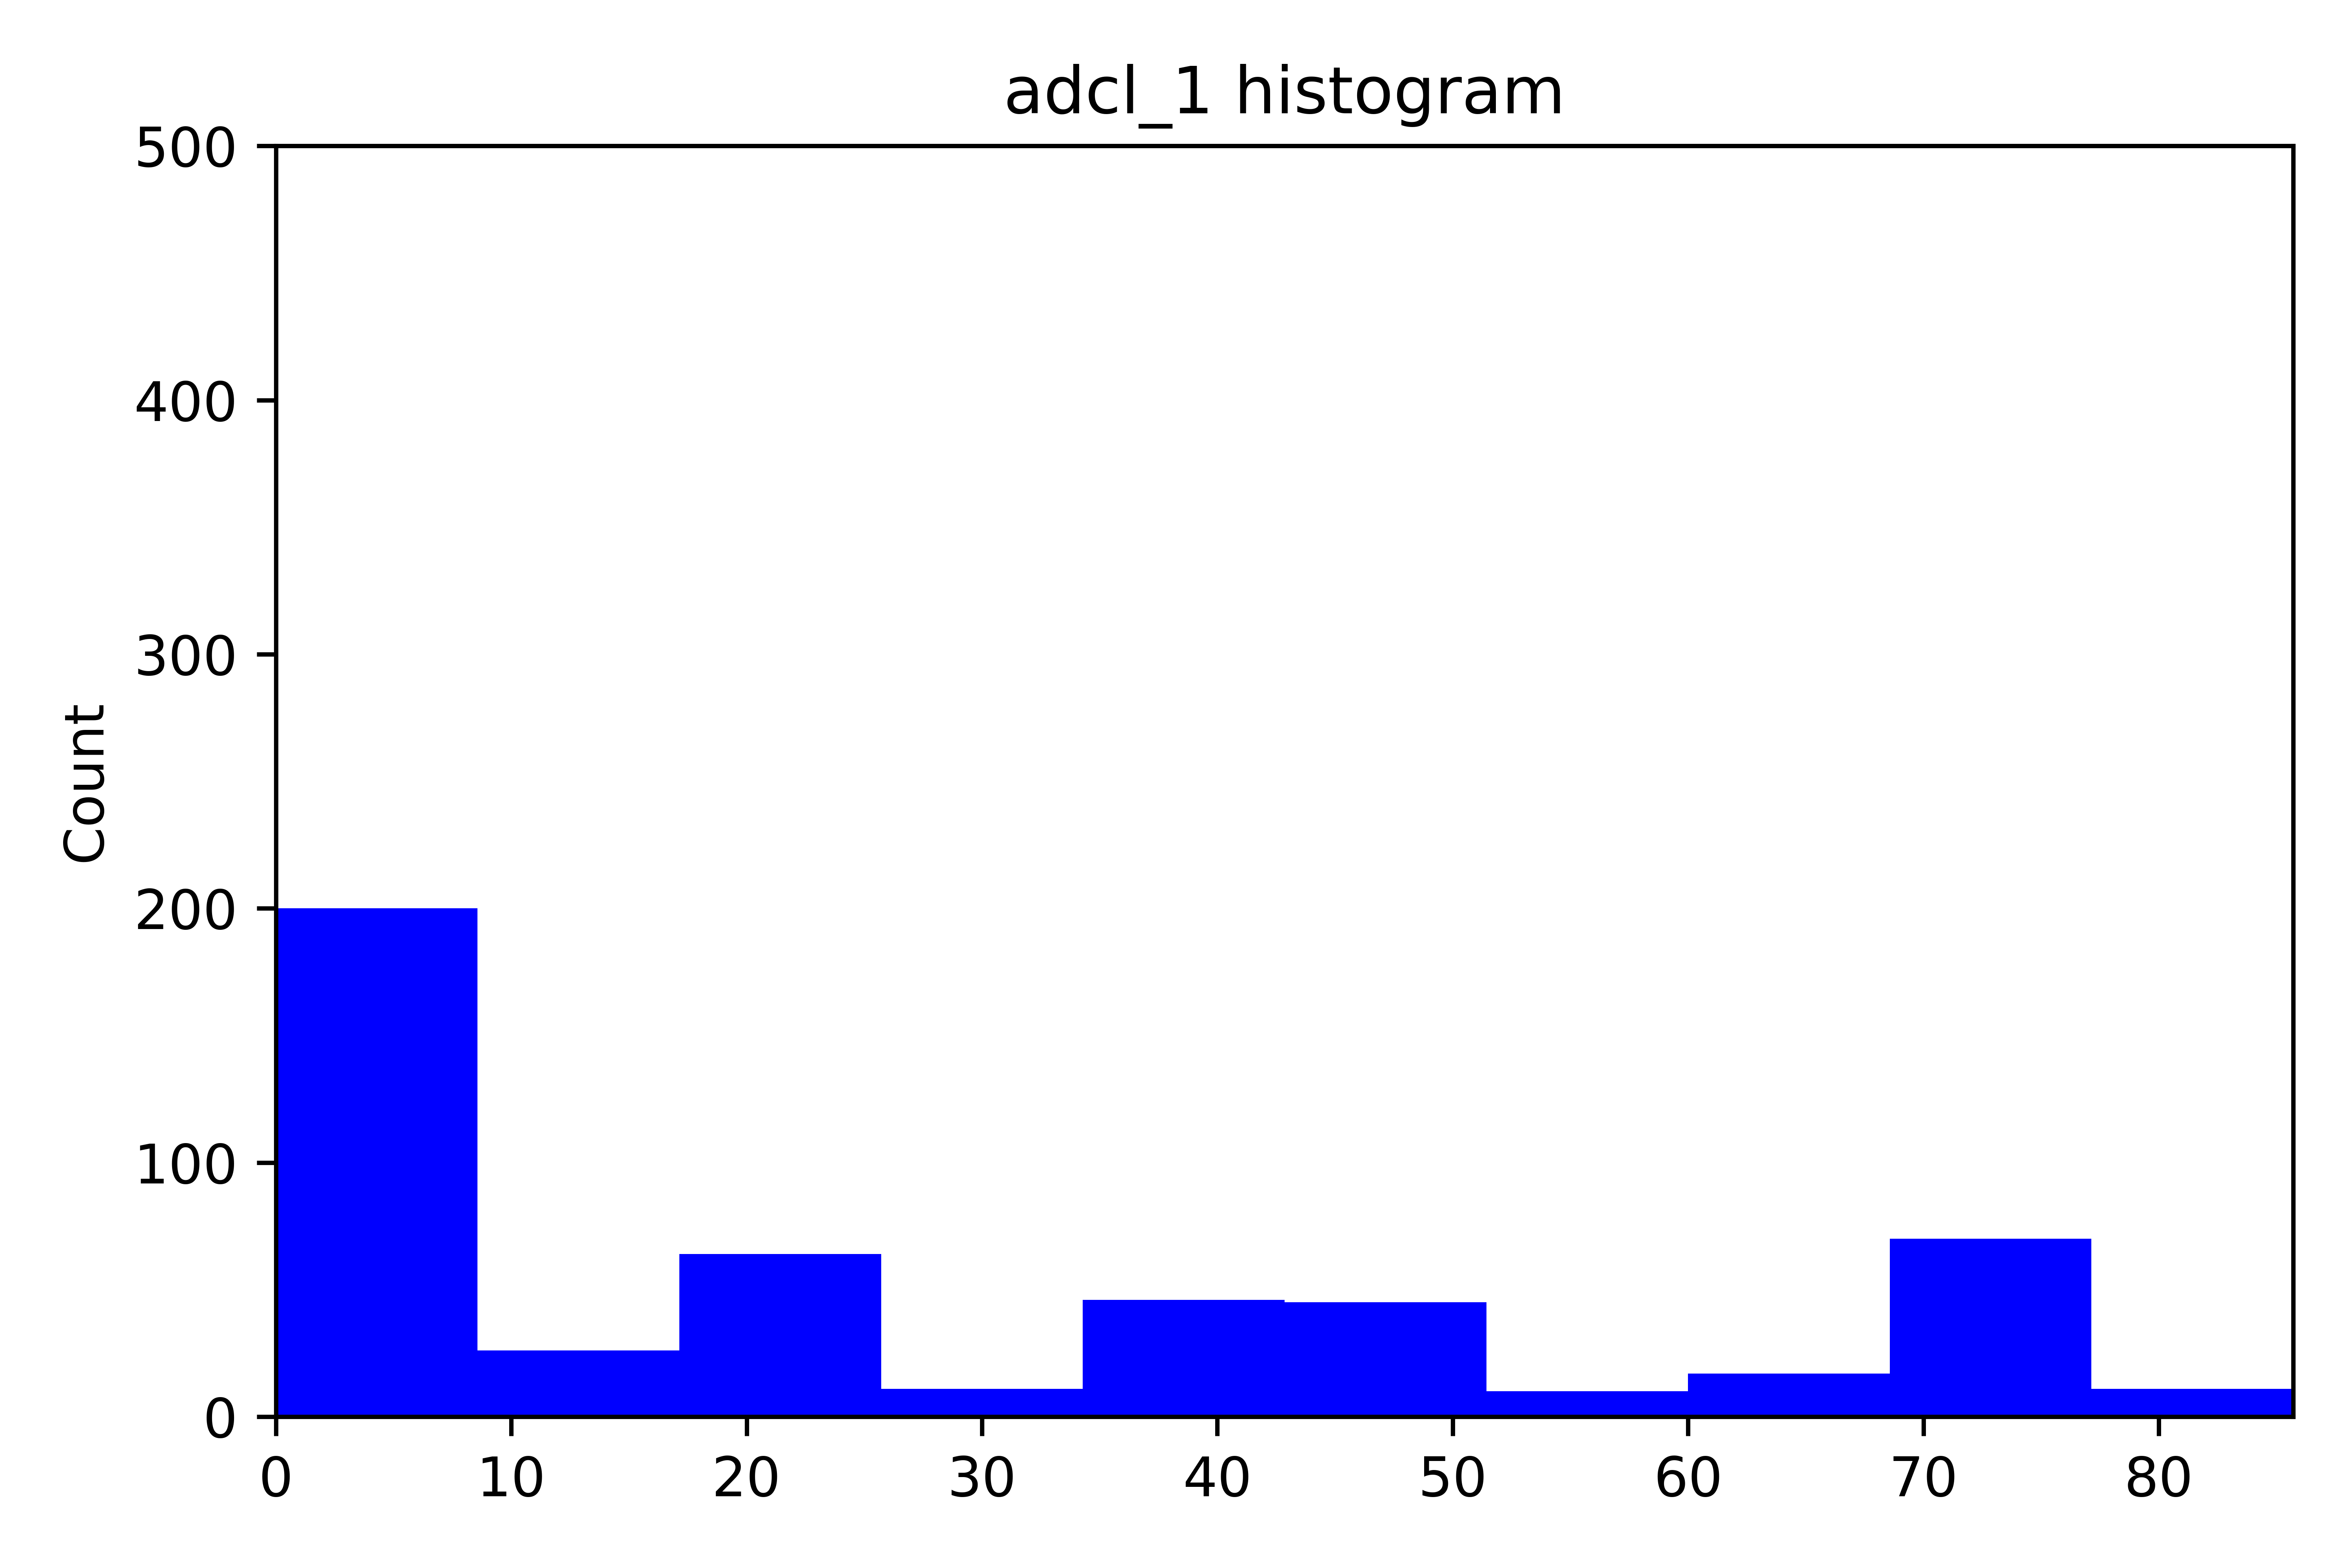
\includegraphics[width=\textwidth, keepaspectratio]{adcl_1-communitylevel.png}\\
	\caption{adcl_1 distribution}
	\label{adcl_1-communitylevel}
\end{figure}

adcl_2 is the median for the dataset whose values is larger than the cutoff value 0.001. The histogram of adcl_2 is shown as in Figure \ref{adcl_2-communitylevel}. \par
\begin{figure}[H]
	\centering
	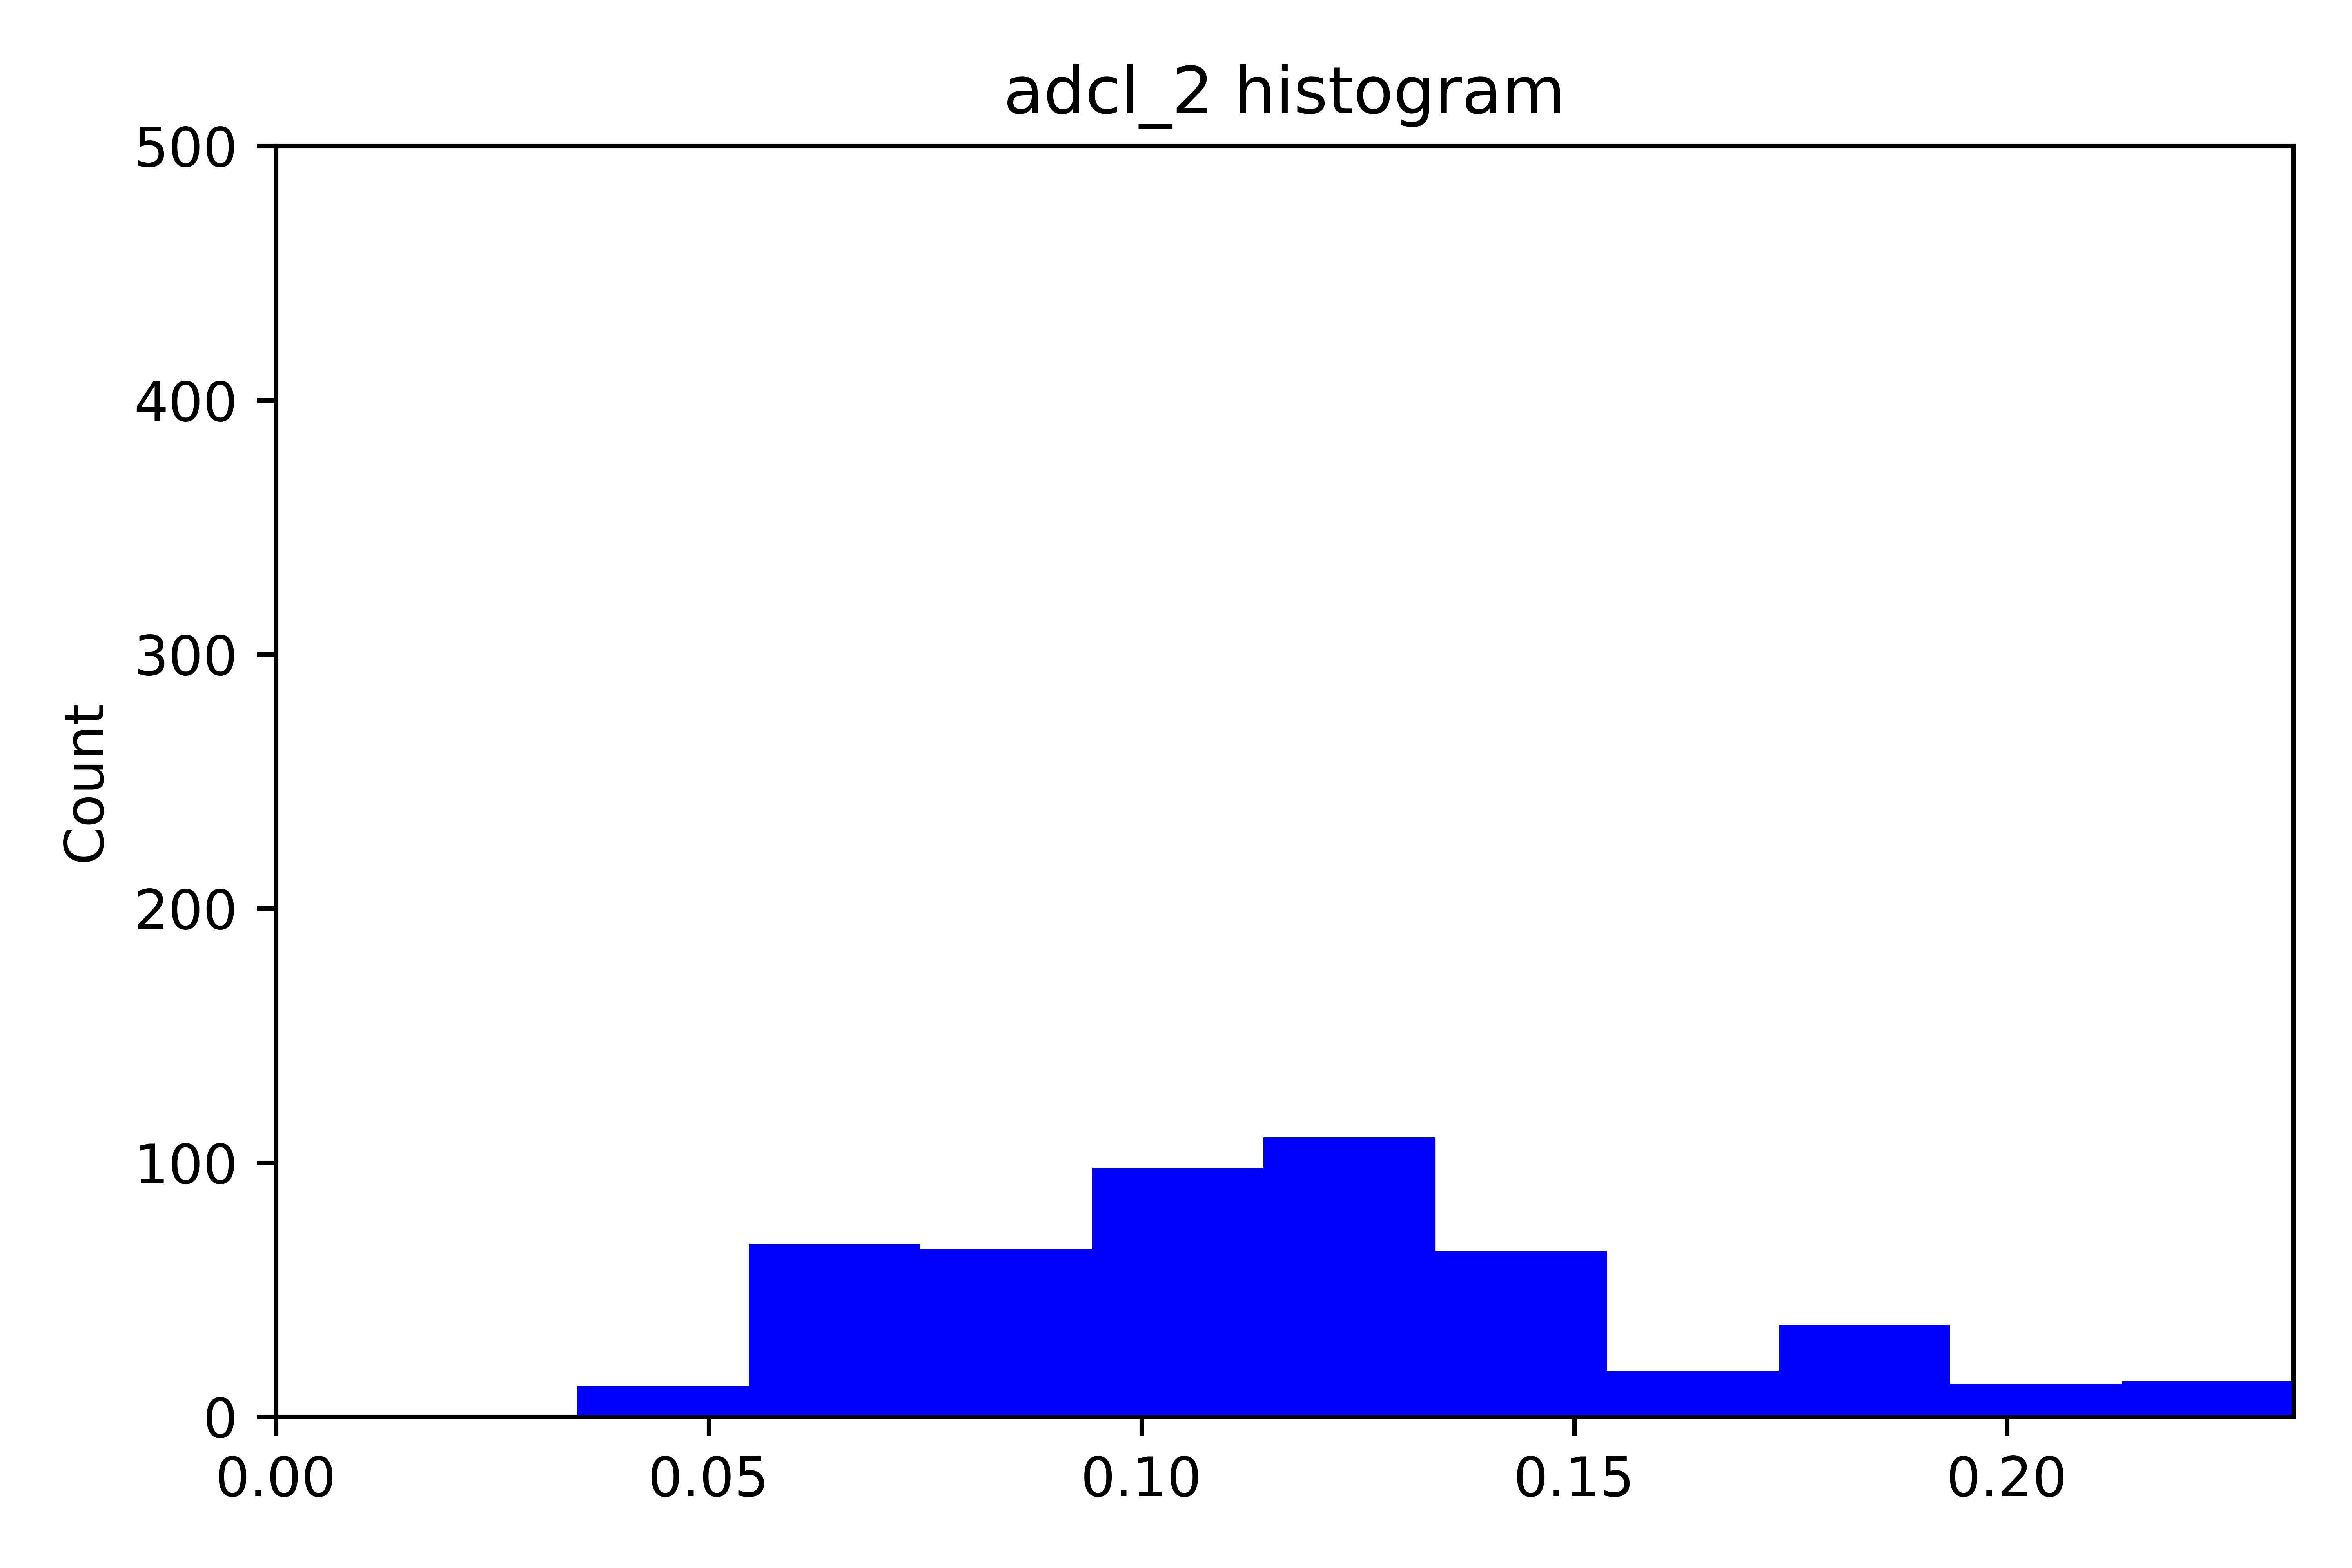
\includegraphics[width=\textwidth, keepaspectratio]{adcl_2-communitylevel.png}\\
	\caption{adcl_2 distribution}
	\label{adcl_2-communitylevel}
\end{figure}
prichness is the percentile at the cutoff value 5, and the histogram of prichness is shown as in Figure \ref{prichness-communitylevel}. \par
\begin{figure}[H]
	\centering
	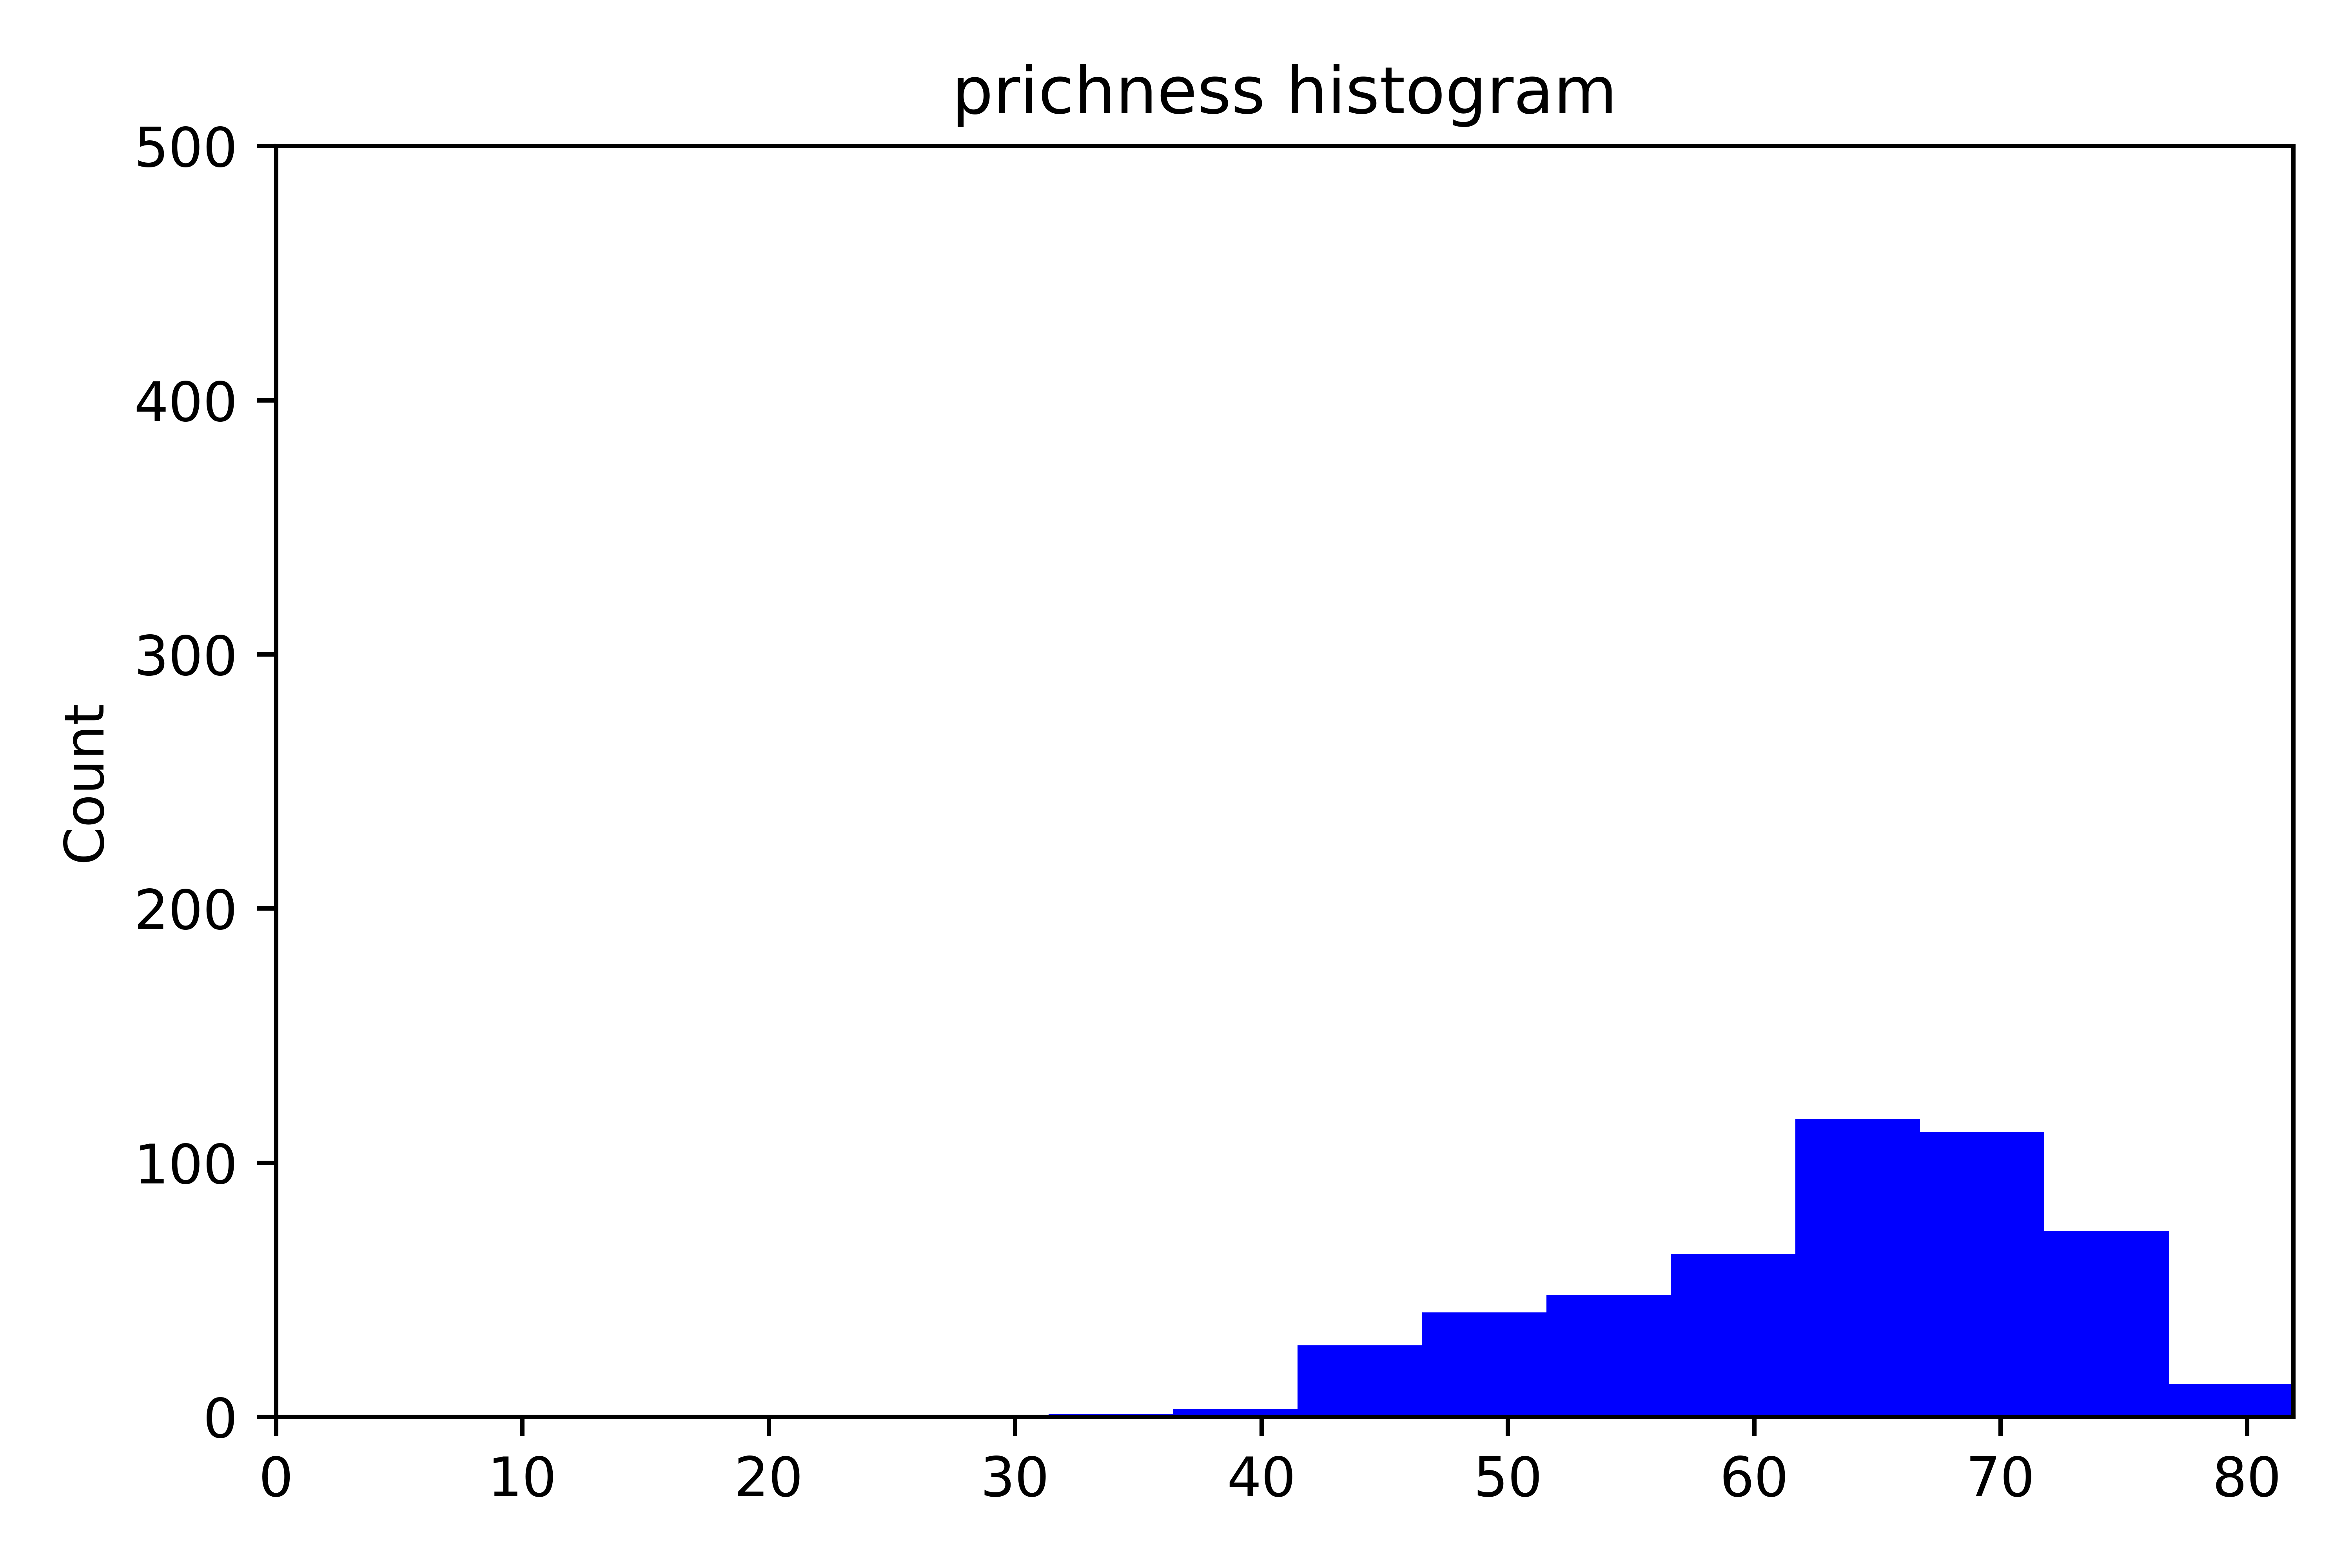
\includegraphics[width=\textwidth, keepaspectratio]{prichness-communitylevel.png}\\
	\caption{prichness distribution}
	\label{prichness-communitylevel}
\end{figure}
edpl_1 is the score at the 75\% for the dataset whose values are larger than the cutoff value 0.1, and the histogram of edpl_1 is shown as in Figure \ref{edpl_1-communitylevel}. \par
\begin{figure}[H]
	\centering
	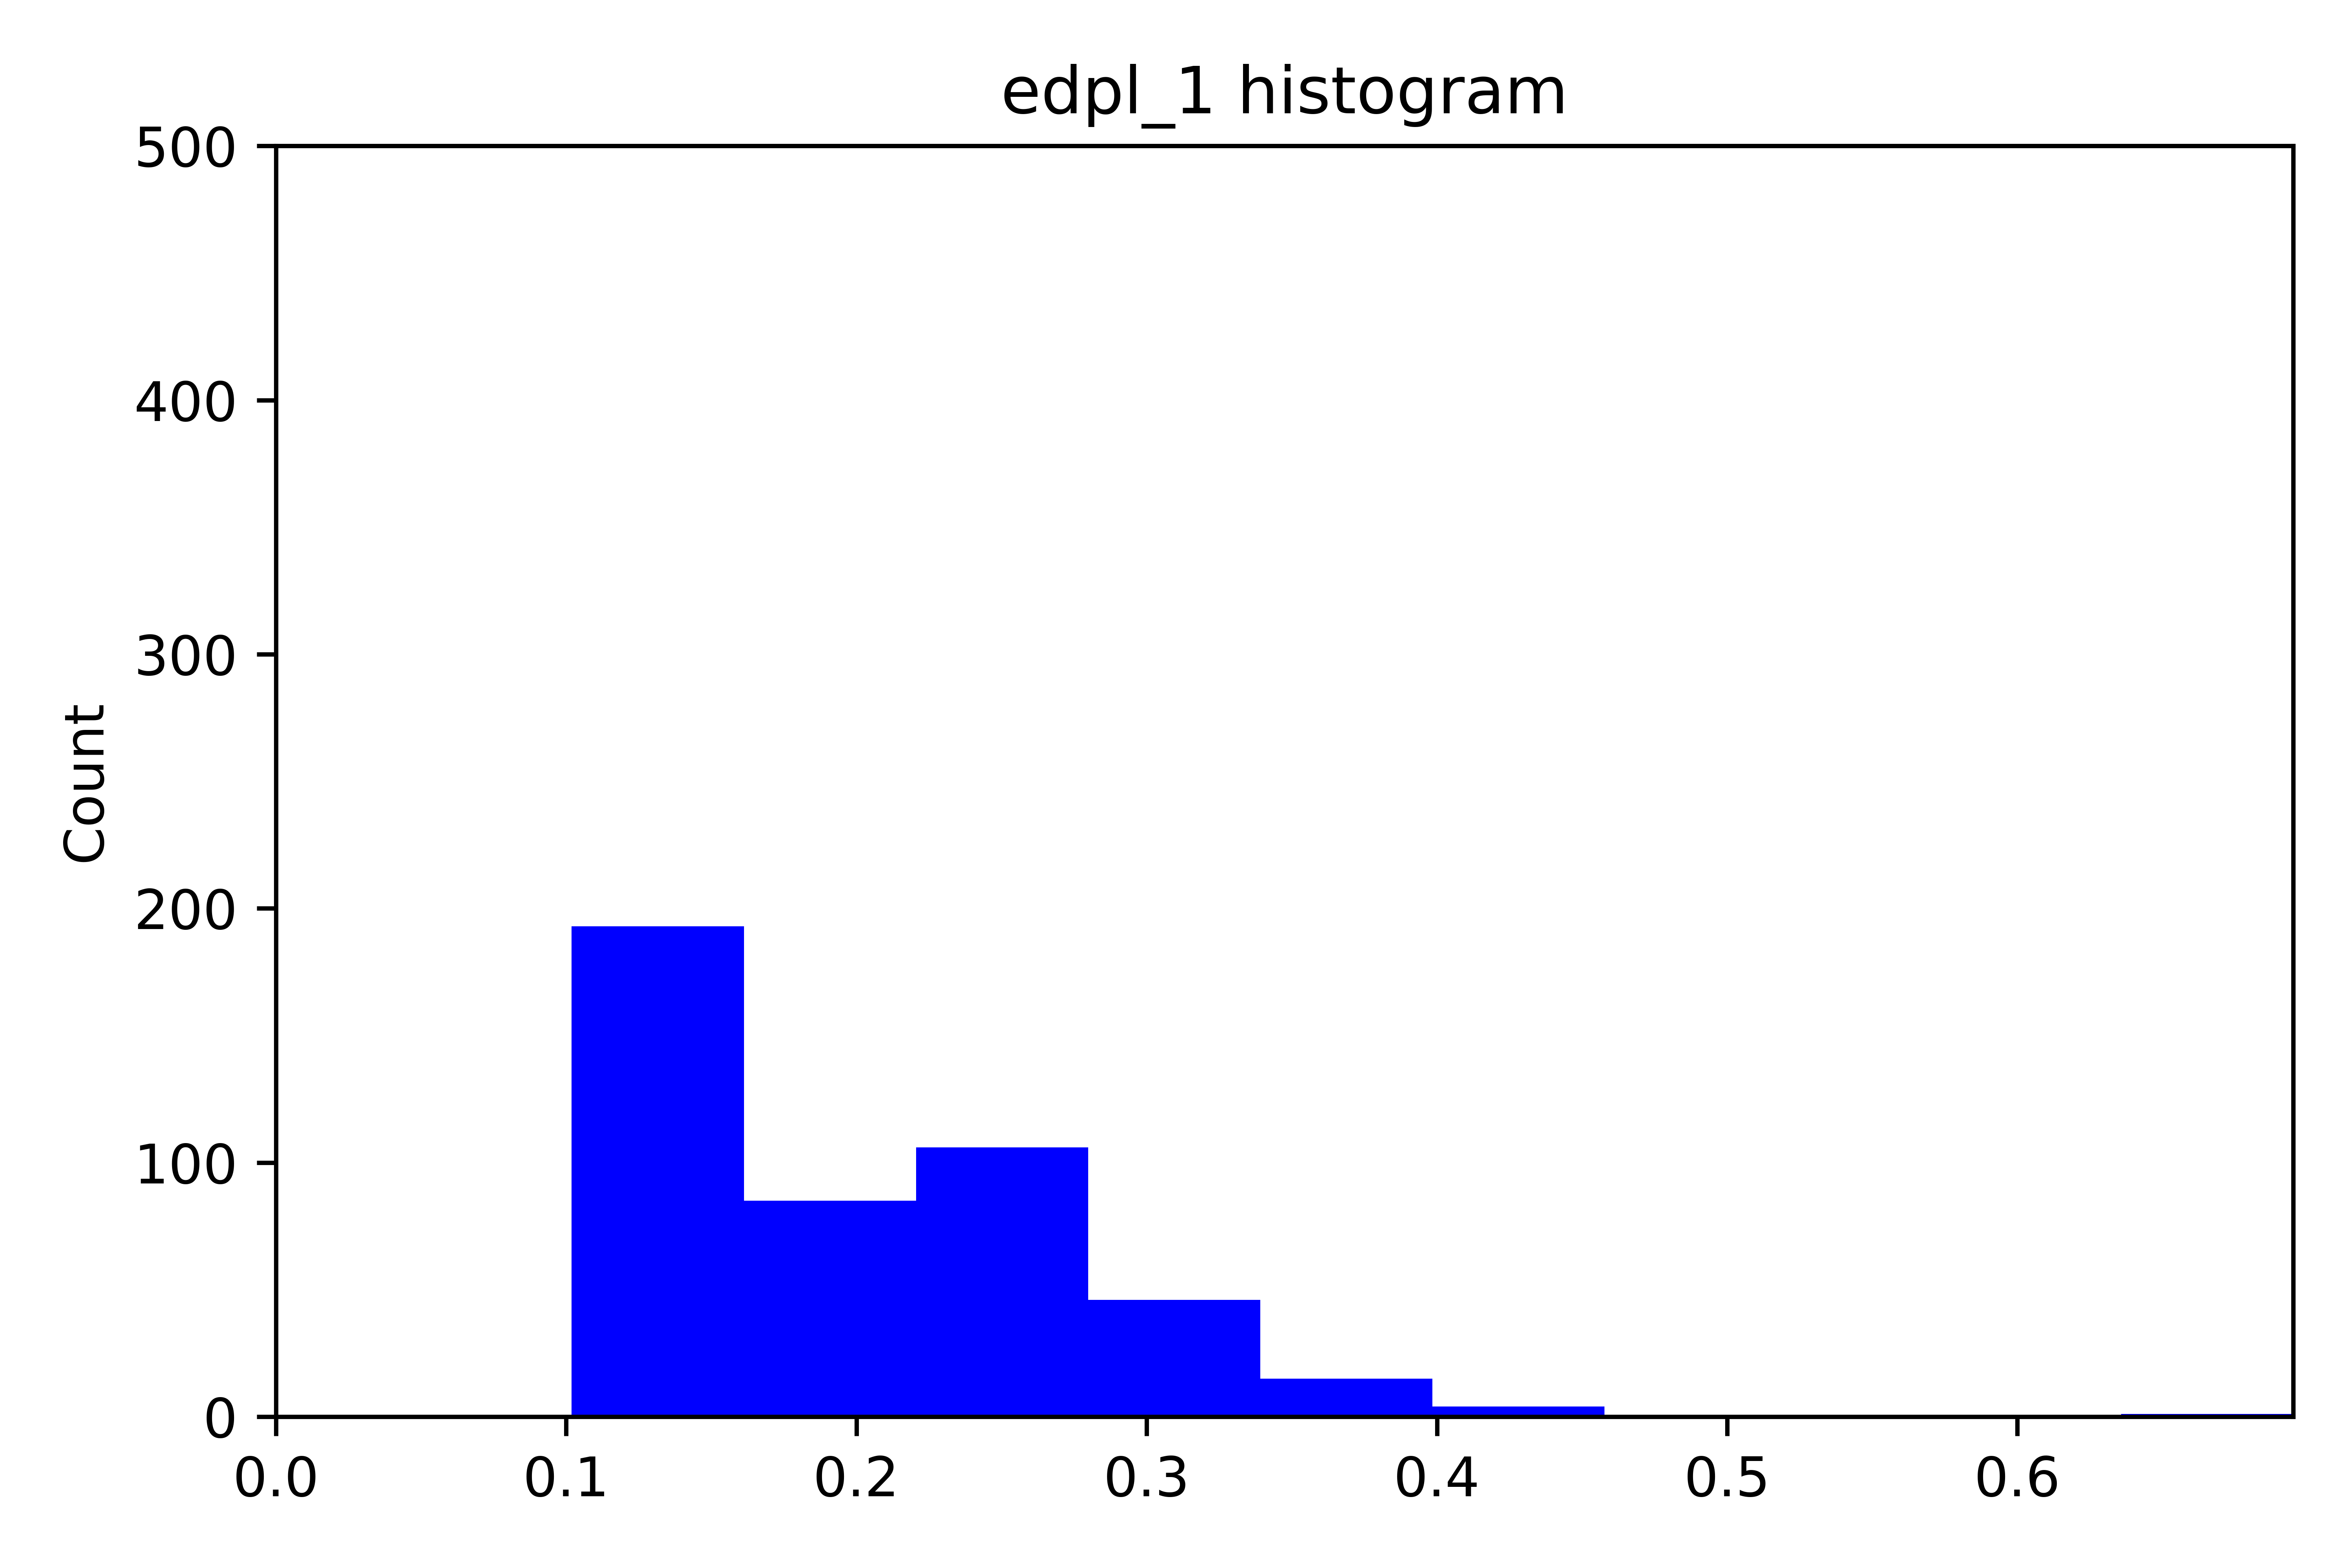
\includegraphics[width=\textwidth, keepaspectratio]{edpl_1-communitylevel.png}\\
	\caption{edpl_1 distribution}
	\label{edpl_1-communitylevel}
\end{figure}
edpl_2 is the score at the 75\% for the dataset whose values are larger than the cutoff value 0.01, and the histogram of edpl_2 is shown as in Figure  \ref{edpl_2-communitylevel}. \par
\begin{figure}[H]
	\centering
	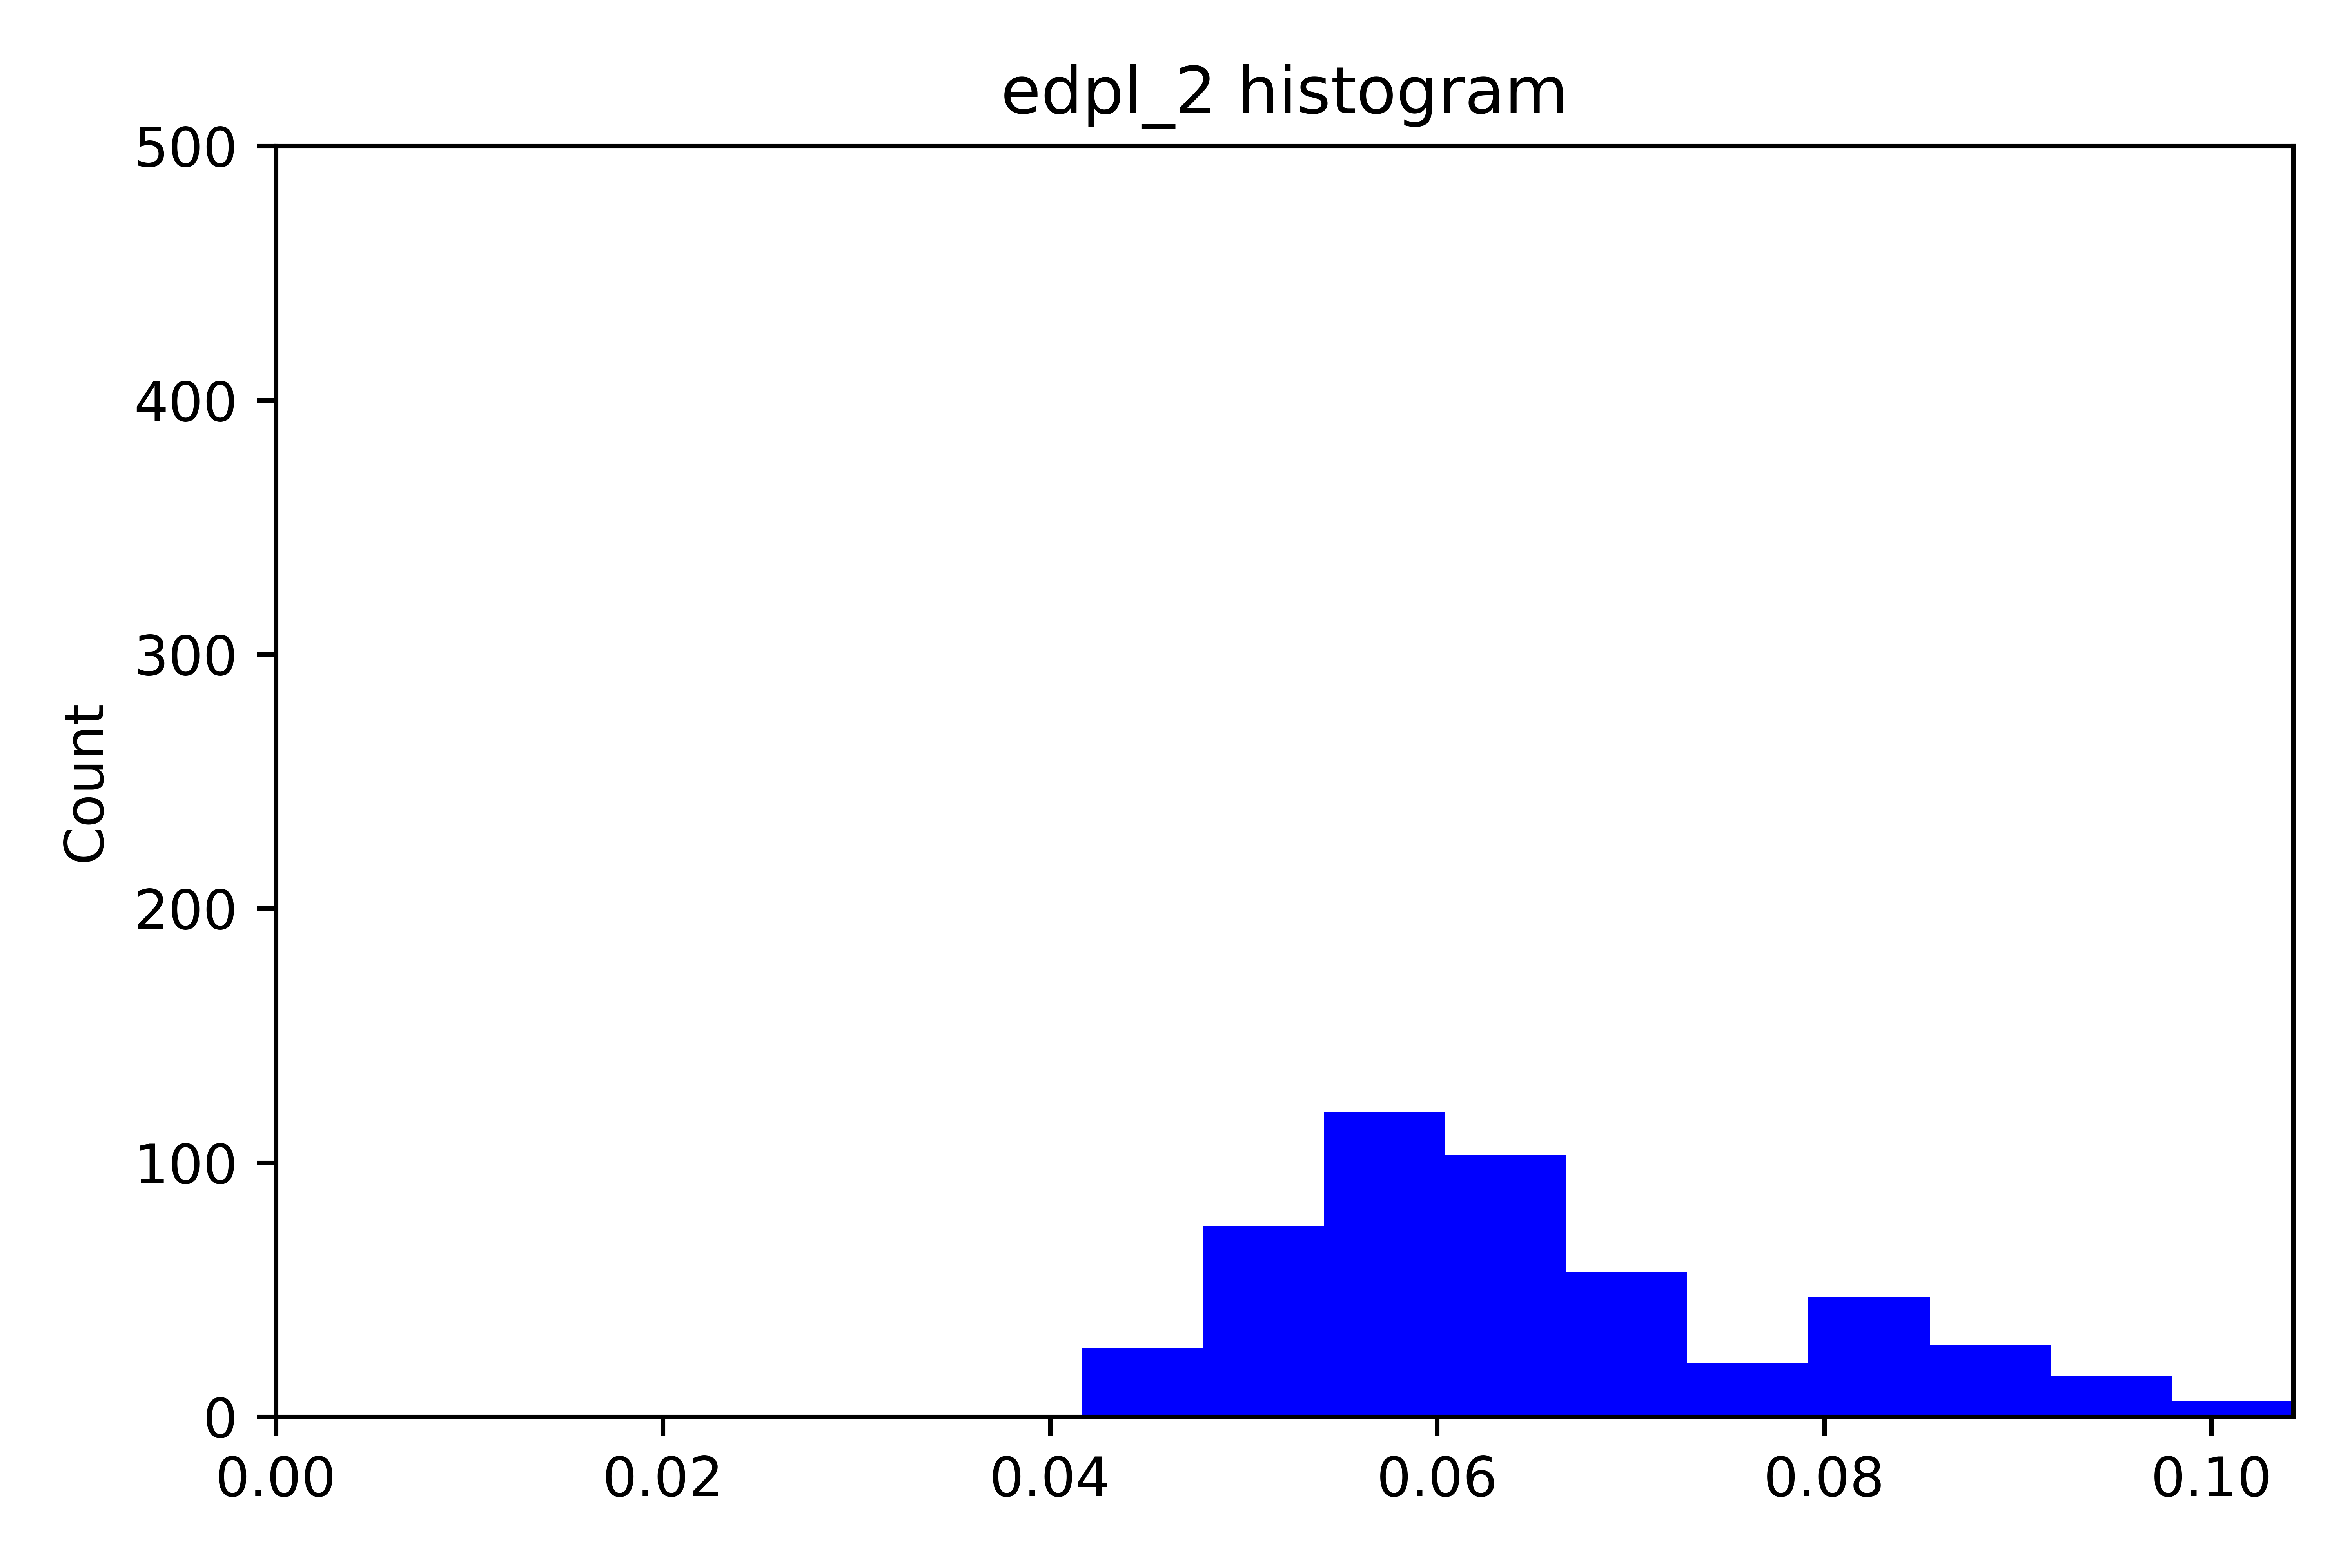
\includegraphics[width=\textwidth, keepaspectratio]{edpl_2-communitylevel.png}\\
	\caption{edpl_2 distribution}
	\label{edpl_2-communitylevel}
\end{figure}
\subsection{Response variables}



\subsubsection{Bray-Curtis Distance}

bcd, shown as in Figure \ref{bcd-communitylevel}. \par
\begin{figure}[H]
	\centering
	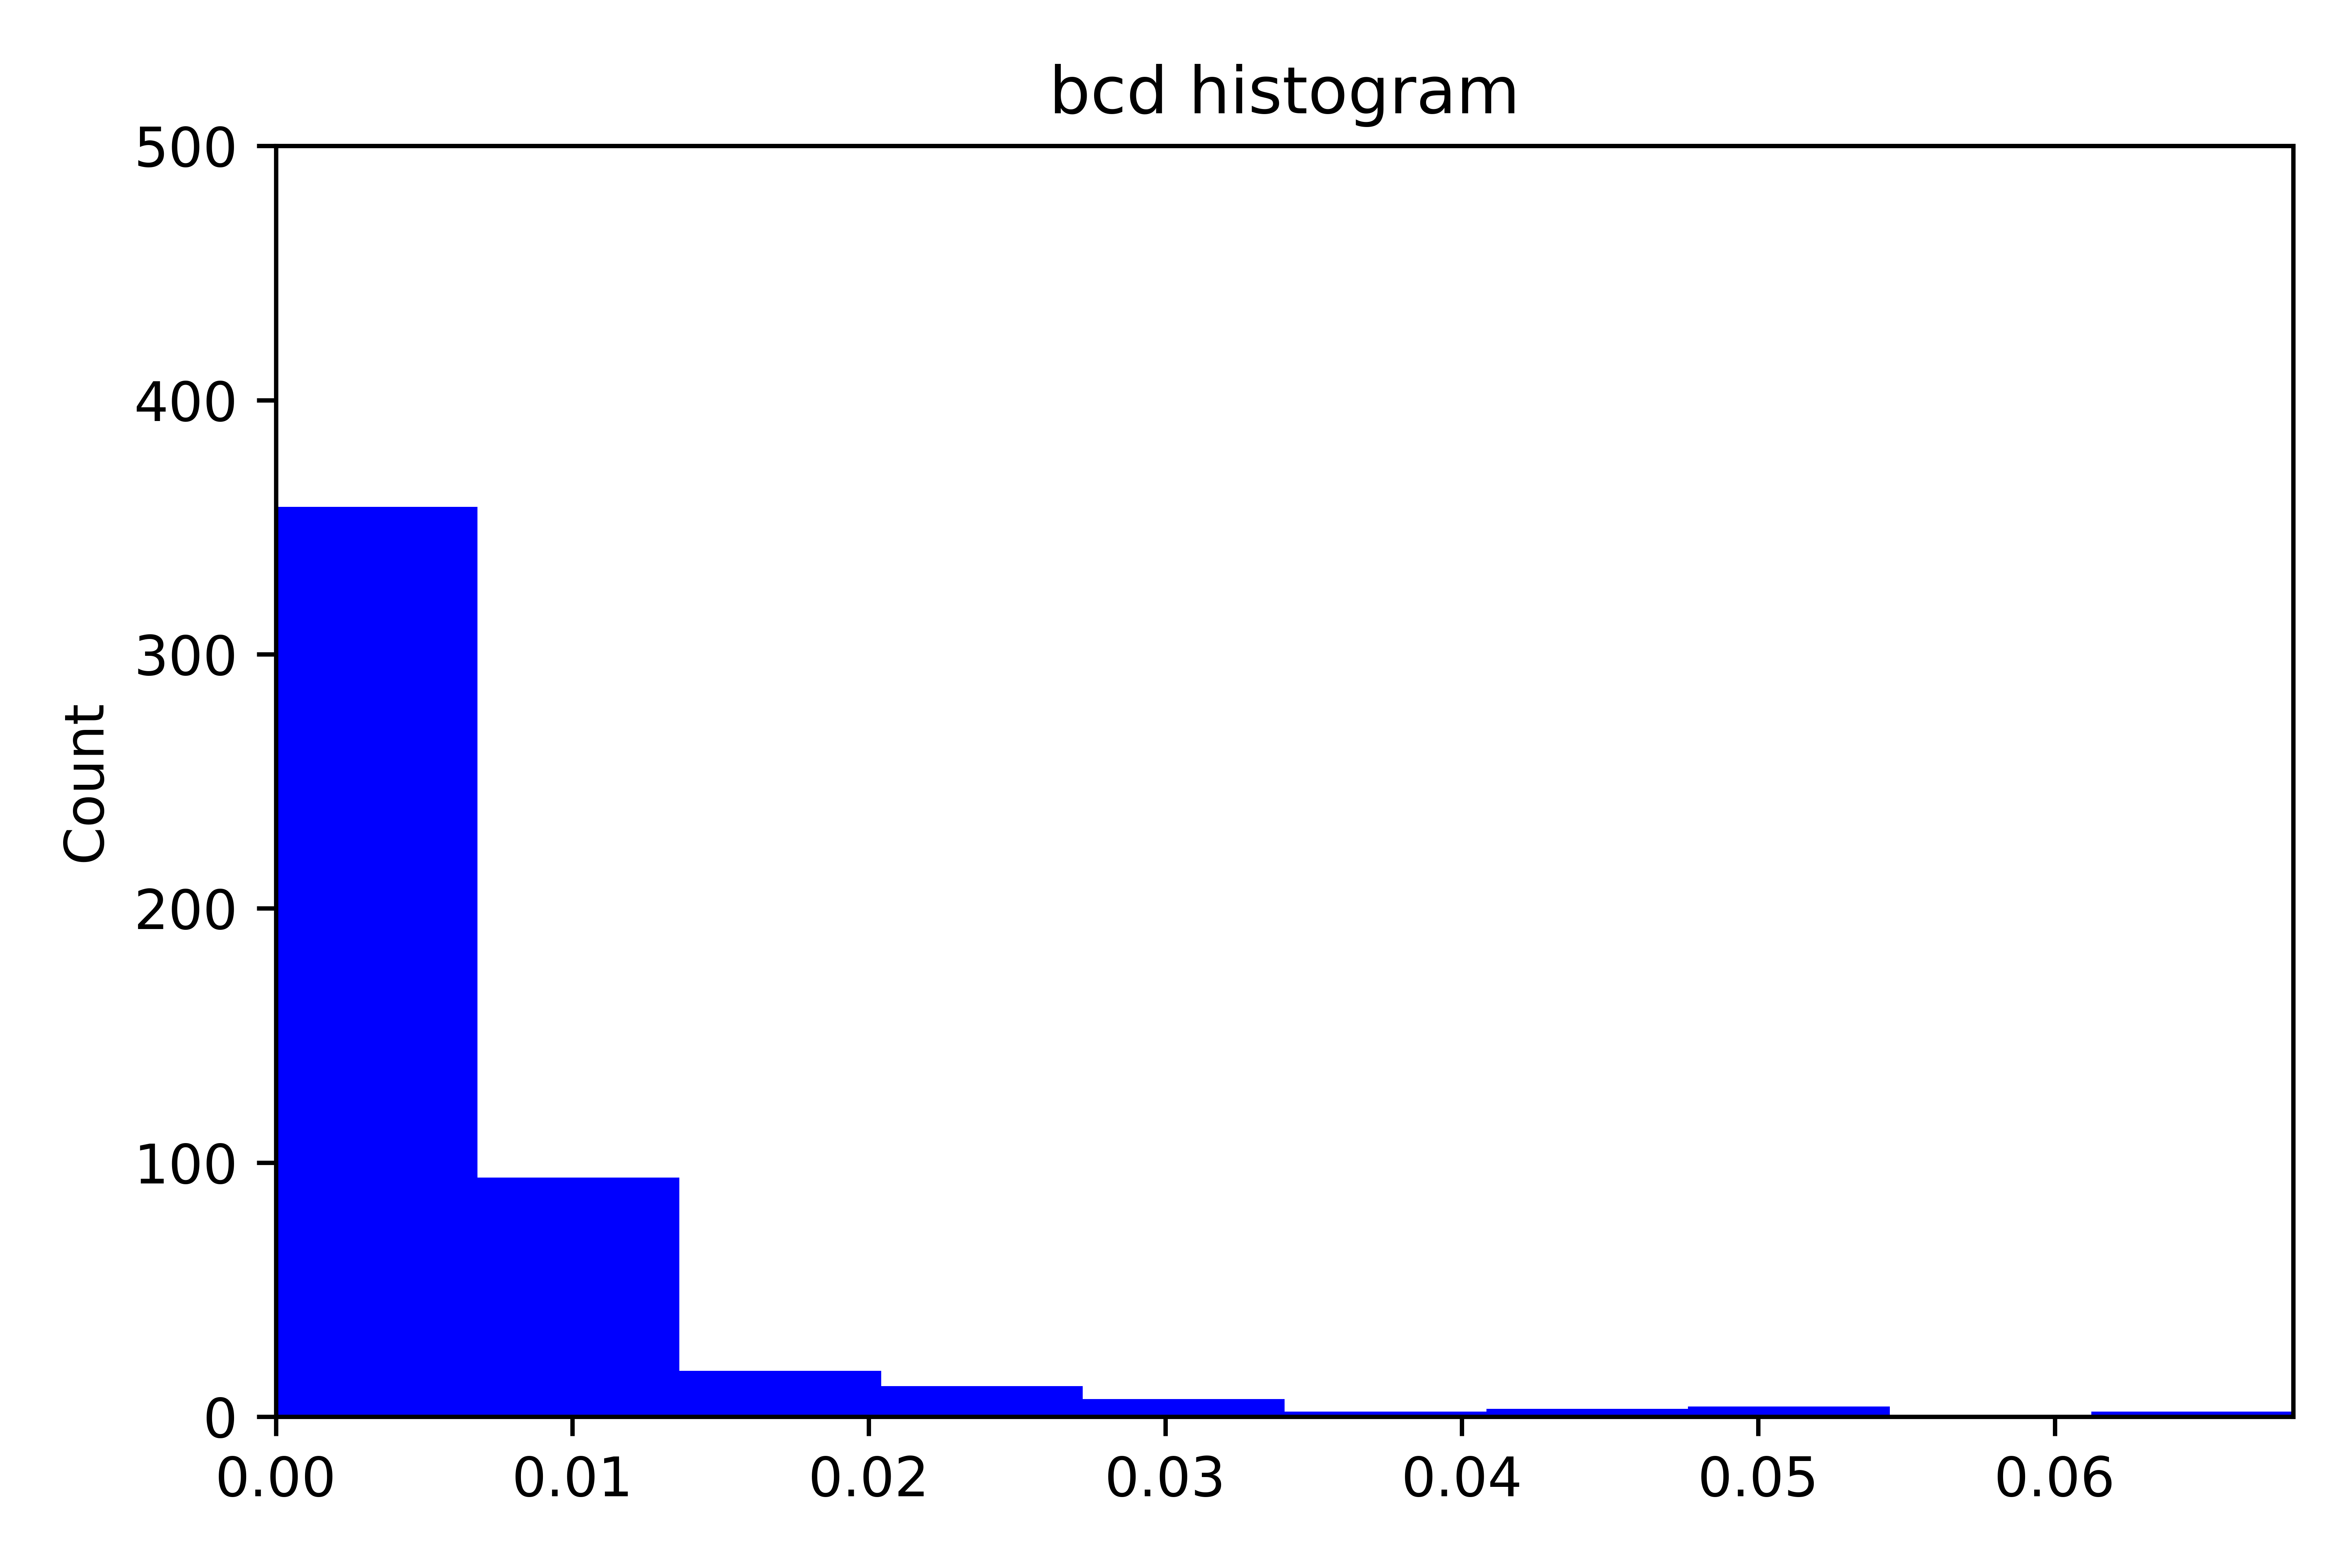
\includegraphics[width=\textwidth, keepaspectratio]{bcd-communitylevel.png}\\
	\caption{bcd distribution}
	\label{bcd-communitylevel}
\end{figure}

\subsubsection{Sensitivity}
sensitivity, shown as in Figure \ref{sensitivity-communitylevel}. \par
\begin{figure}[H]
	\centering
	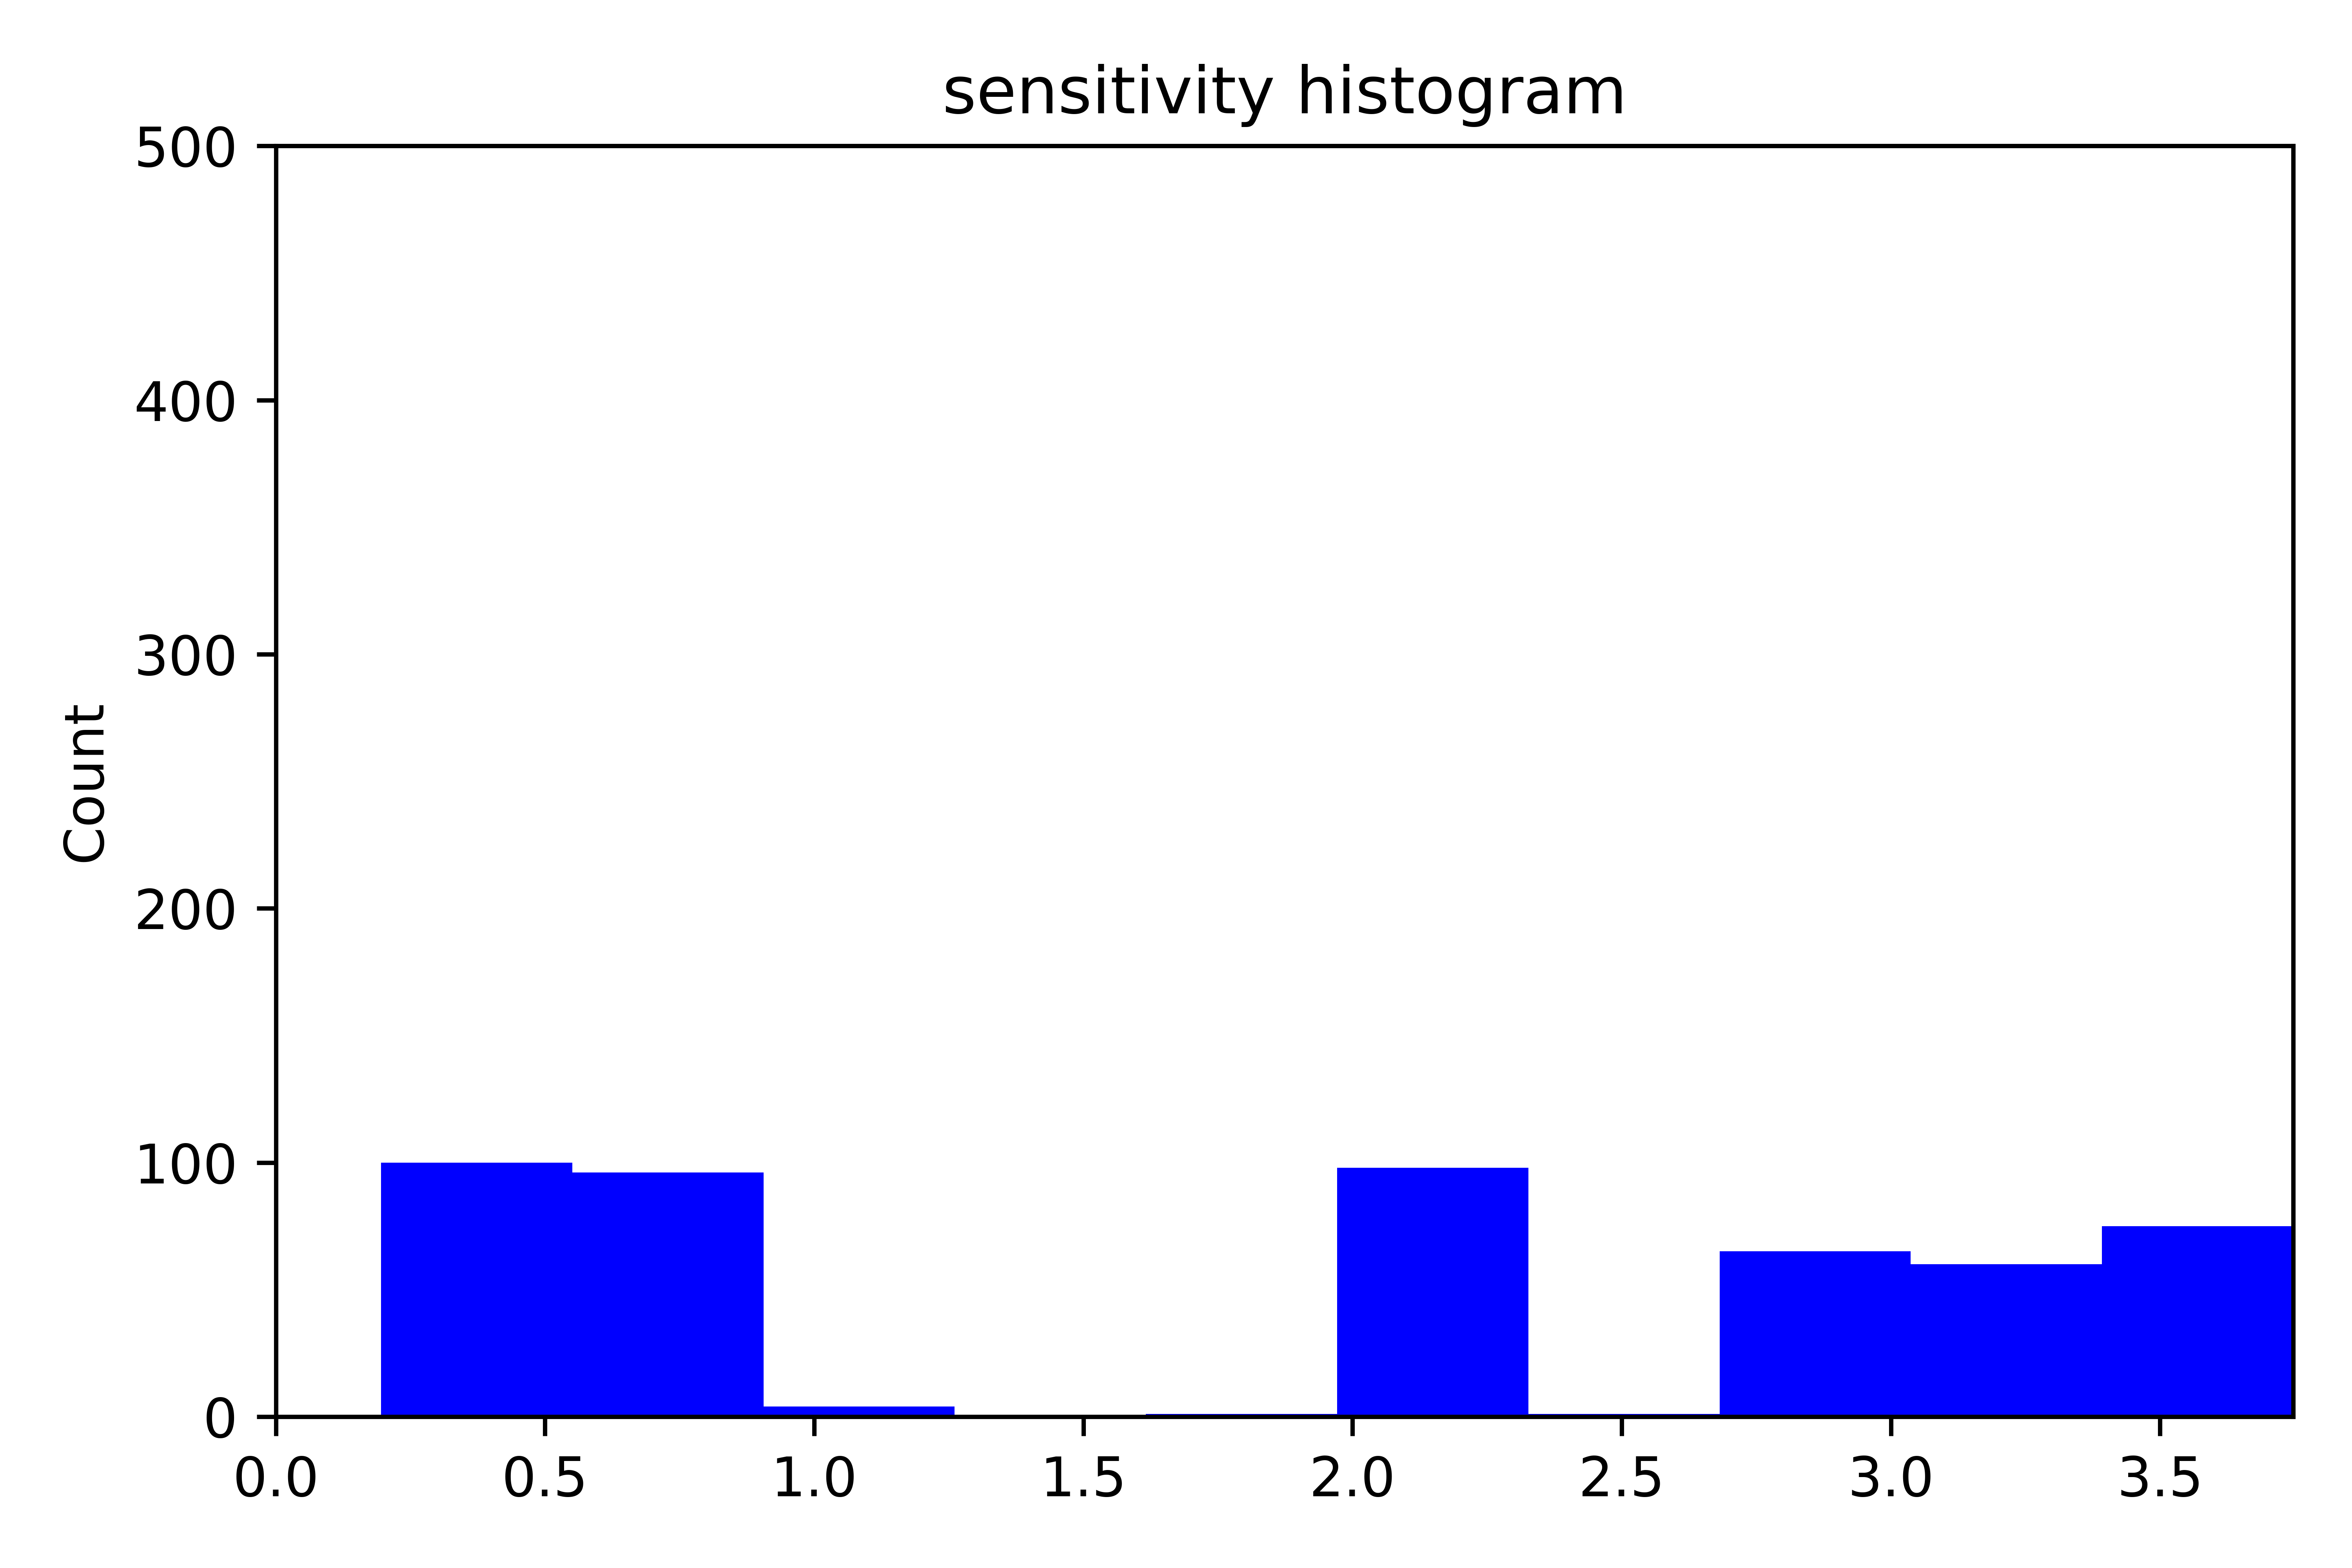
\includegraphics[width=\textwidth, keepaspectratio]{sensitivity-communitylevel.png}\\
	\caption{sensitivity distribution}
	\label{sensitivity-communitylevel}
\end{figure}

\subsubsection{Correlation on community level}
pairplot is shown in Figure \ref{pairplot-communitylevel}.\par
\begin{figure}[H]
	\centering
	\includegraphics[width=\textwidth, keepaspectratio]{pairplot-community.png}\\
	\caption{pairplot}
	\label{pairplot-communitylevel}
\end{figure}
linear regression with the sensitivity as the response variable was performed and the coefficients are shown in Table \ref{Tab:corresensitivity}. \par
\begin{table}[ht]
\caption{Correlation between sensitivity and pplacer stats}
\begin{tabular}{llllll}
\hline
            & Estimate &Std. Error &t value &Pr(>|t|) & Significance    \\
            \hline
(Intercept) & 1.381843 &  0.261490 &  5.284 &1.98e-07 &*** \\
adcl_1      & 0.028468 &  0.001007 & 28.267 & < 2e-16 &*** \\
adcl_2      &-9.805436 &  0.789221 &-12.424 & < 2e-16 &*** \\
prichness   & 0.004077 &  0.002668 &  1.528 & 0.12717 &    \\
edpl_1      & 0.619069 &  0.212299 &  2.916 & 0.00372 &**  \\
edpl_2      & 8.567660 &  1.195613 &  7.166 &3.24e-12 &*** \\
\hline
\end{tabular}
\label{Tab:corresensitivity}
\end{table}

linear regression with the bray-curtis distance as the response variable was performed and the coefficients are shown in Table \ref{Tab:correbcd}. \par
\begin{table}[ht]
\caption{Correlation between Bray-Curtis distance and pplacer stats}
\begin{tabular}{llllll}
\hline
            & Estimate &Std. Error &t value &Pr(>|t|) & Significance    \\
            \hline
(Intercept)&  3.391e-03 & 7.123e-03 &  0.476 &  0.6342&  \\
adcl_1     & -5.081e-05 & 2.743e-05 & -1.852 &  0.0647& .\\
adcl_2     &  2.487e-02 & 2.150e-02 &  1.157 &  0.2479&  \\
prichness  &  5.880e-05 & 7.267e-05 &  0.809 &  0.4188&  \\
edpl_1     & -3.066e-03 & 5.783e-03 & -0.530 &  0.5962&  \\
edpl_2     & -4.438e-02 & 3.257e-02 & -1.363 &  0.1736& \\
\hline
\end{tabular}
\label{Tab:correbcd}
\end{table}
linear regression with the sensitivity and Bray-Curtis distance(bcd) as the response variable was performed and the coefficients are shown in Table \ref{Tab:correall}. \par
\begin{table}[ht]
\caption{Repeat measures mixed model}
\begin{tabular}{llllll}
\hline
           & Estimate &Std. Error &t value &R2m&R2c \\
           \hline
(Intercept)&0.7382749 & 0.0288578 &  25.58 & & \\
adcl_1     &0.0425100 & 0.0007366 &  57.71 &0.8696908	&0.8696908\\
(Intercept)&  5.10618 &   0.07838 &  65.15&  & \\
adcl_2     &-26.70134 &   0.62471 & -42.74 &0.7854565	&0.7854565\\
(Intercept)&-4.090738 &  0.264176 & -15.48& & \\
prichness  & 0.095724 &  0.004148 &  23.08 &0.5162433	&0.5162433\\
(Intercept)&  1.3142  &   0.1487  & 8.838& & \\
edpl_1     &  3.7171  &   0.7042  & 5.279 &0.05843436	&0.05843436\\
(Intercept)&  1.0269  &   0.2721  & 3.774& & \\
edpl_2     & 14.0654  &   4.1047  & 3.427 &0.02299017	&0.02299017\\
(Intercept)& 7.627e-03&  6.964e-04&  10.952& & \\
adcl_1     &-7.933e-05&  1.287e-05&  -6.165&0.05247357	&0.3144885\\
(Intercept)&-0.001447 &  0.001174 & -1.233& & \\
adcl_2     & 0.057609 &  0.008559 &  6.731 &0.06345559	&0.3228208\\
(Intercept)& 1.647e-02&  2.540e-03&   6.485& & \\
prichness  &-1.760e-04&  3.919e-05&  -4.490& 0.03018458	&0.2874114\\
(Intercept)& 0.006099 &  0.001173 &  5.198& & \\
edpl_1     &-0.005574 &  0.005153 & -1.082 &0.00221097	&0.2554322\\
(Intercept)& 0.009647 &  0.001979 &  4.874& & \\
edpl_2     &-0.065649 &  0.029077 & -2.258&0.008691836	&0.2581638\\
\hline
\end{tabular}
\label{Tab:correall}
\end{table}

\section{Individual level}

\subsection{Independent variables}

adcl, shown as in Figure \ref{adcl} \par
\begin{figure}[H]
	\centering
	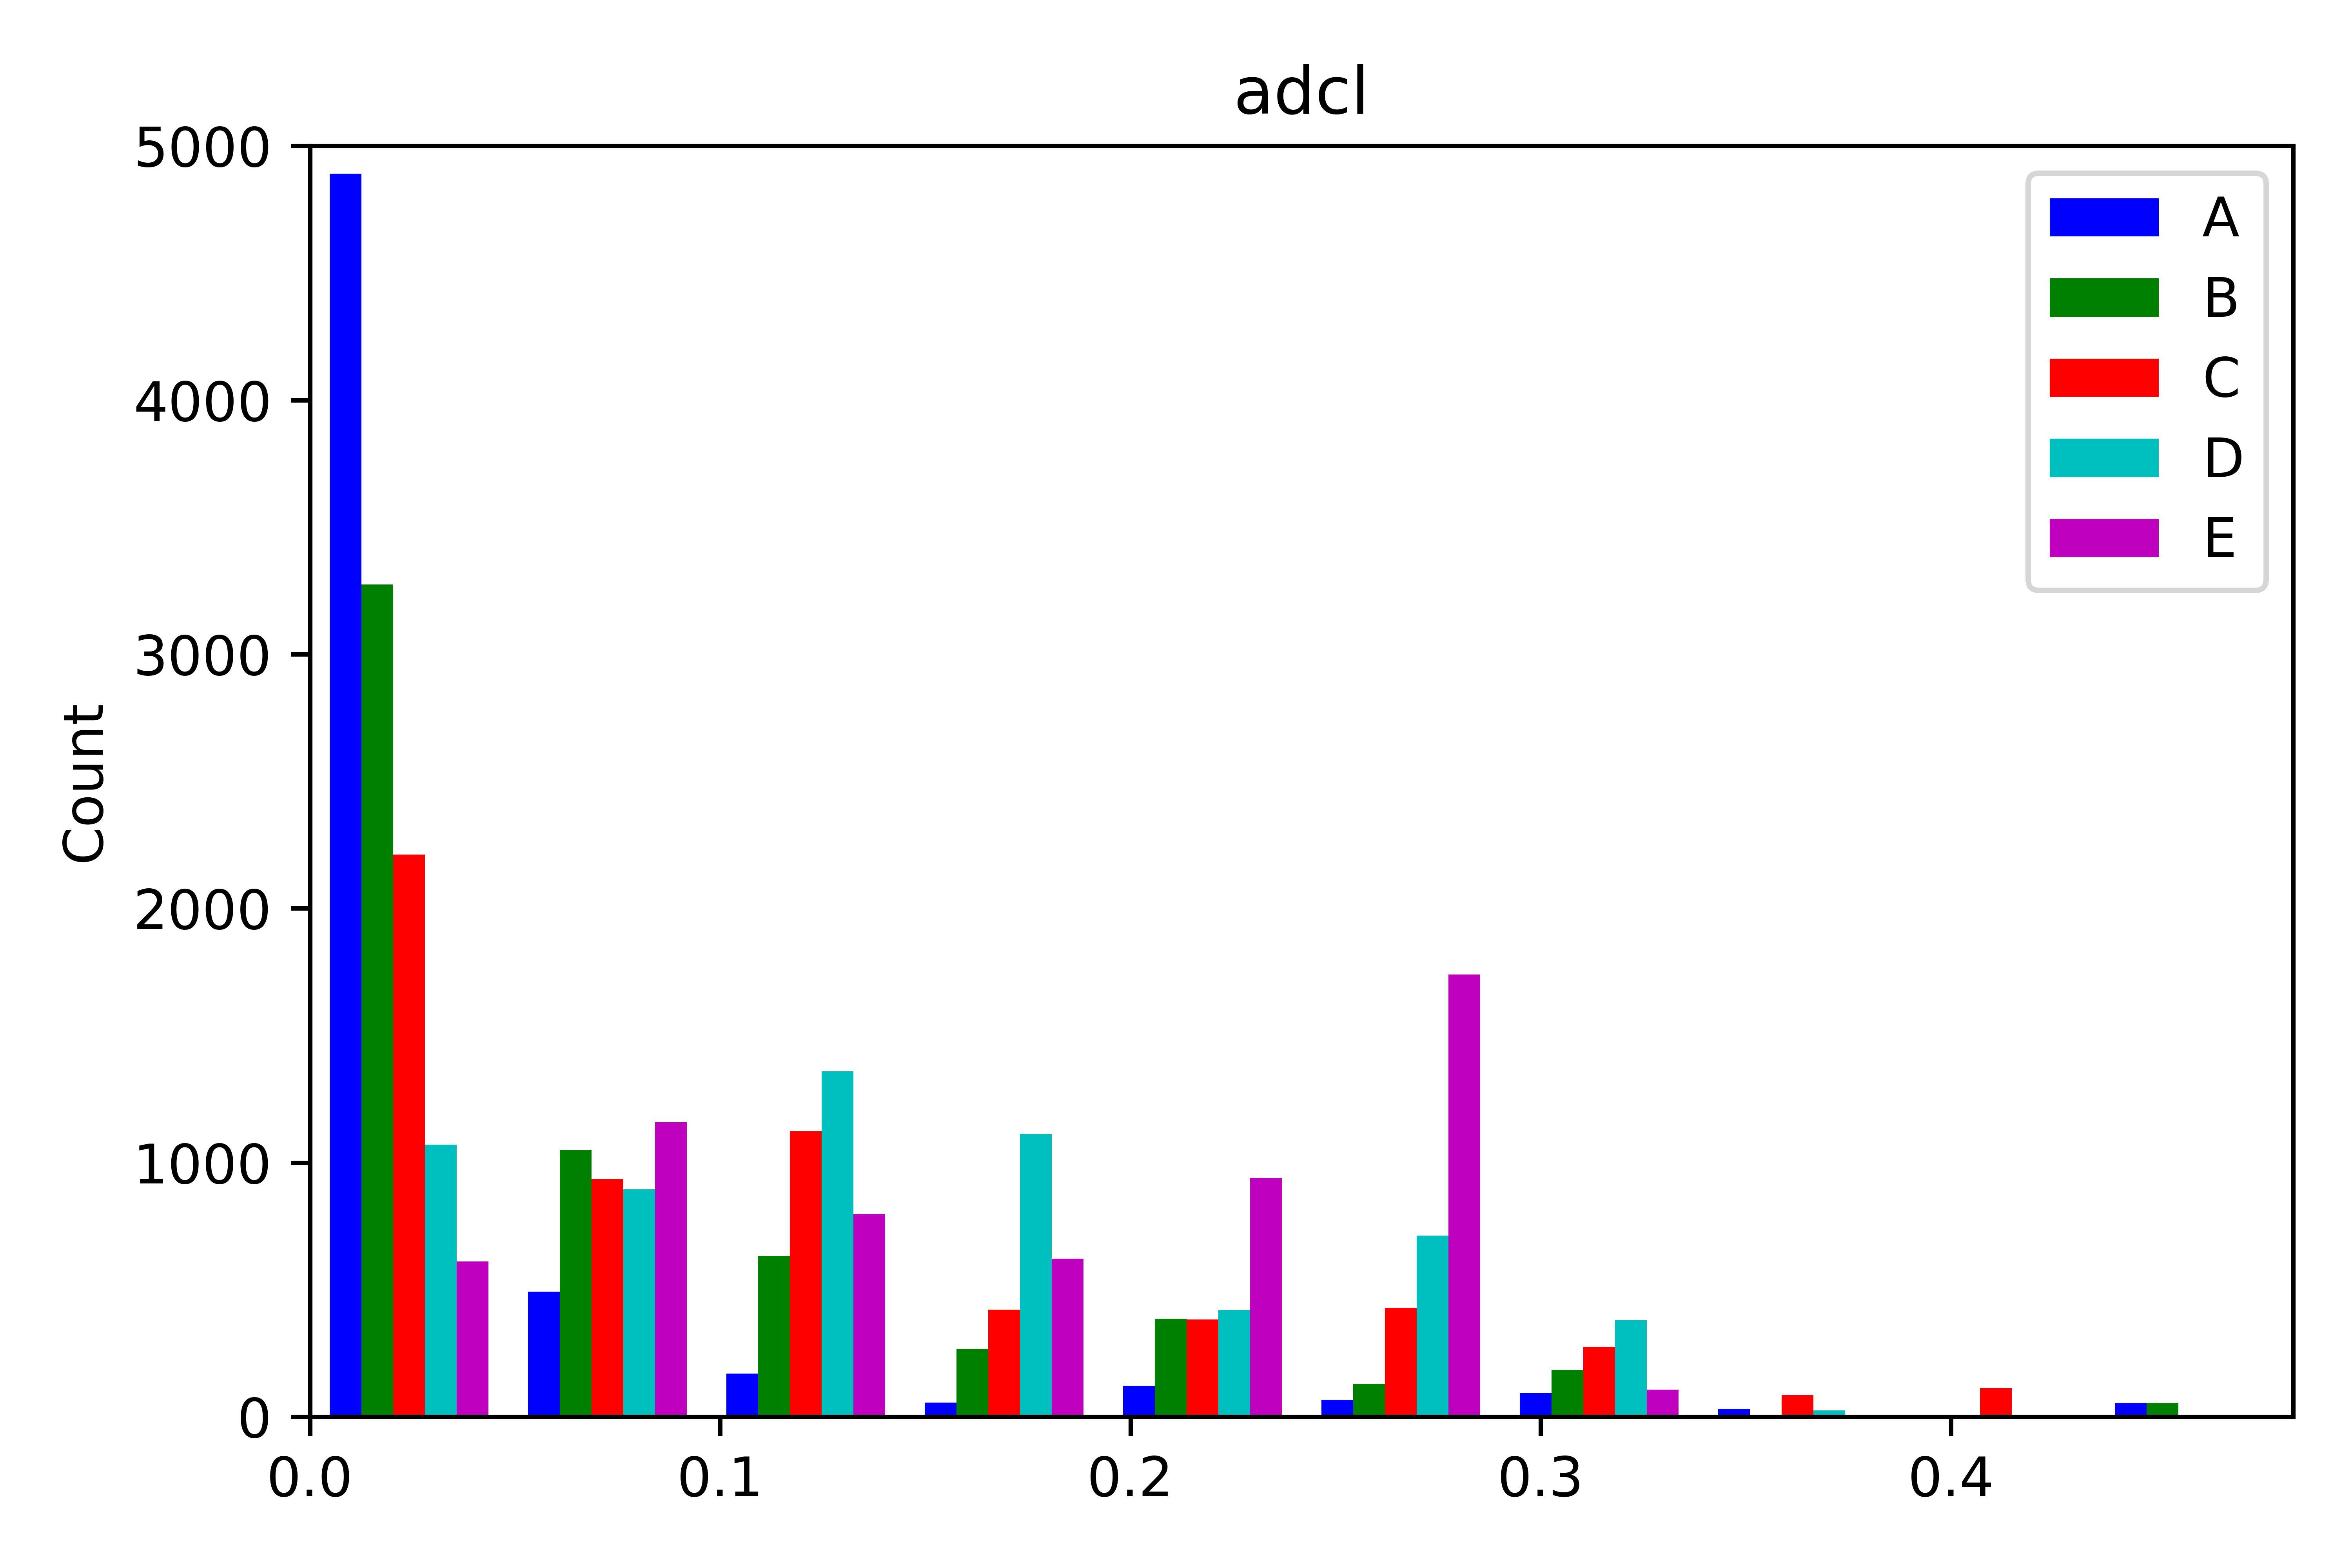
\includegraphics[width=\textwidth, keepaspectratio]{adcl.png}\\
	\caption{adcl distribution}
	\label{adcl}
\end{figure}



edpl, shown as in Figure \ref{edpl} \par
\begin{figure}[H]
	\centering
	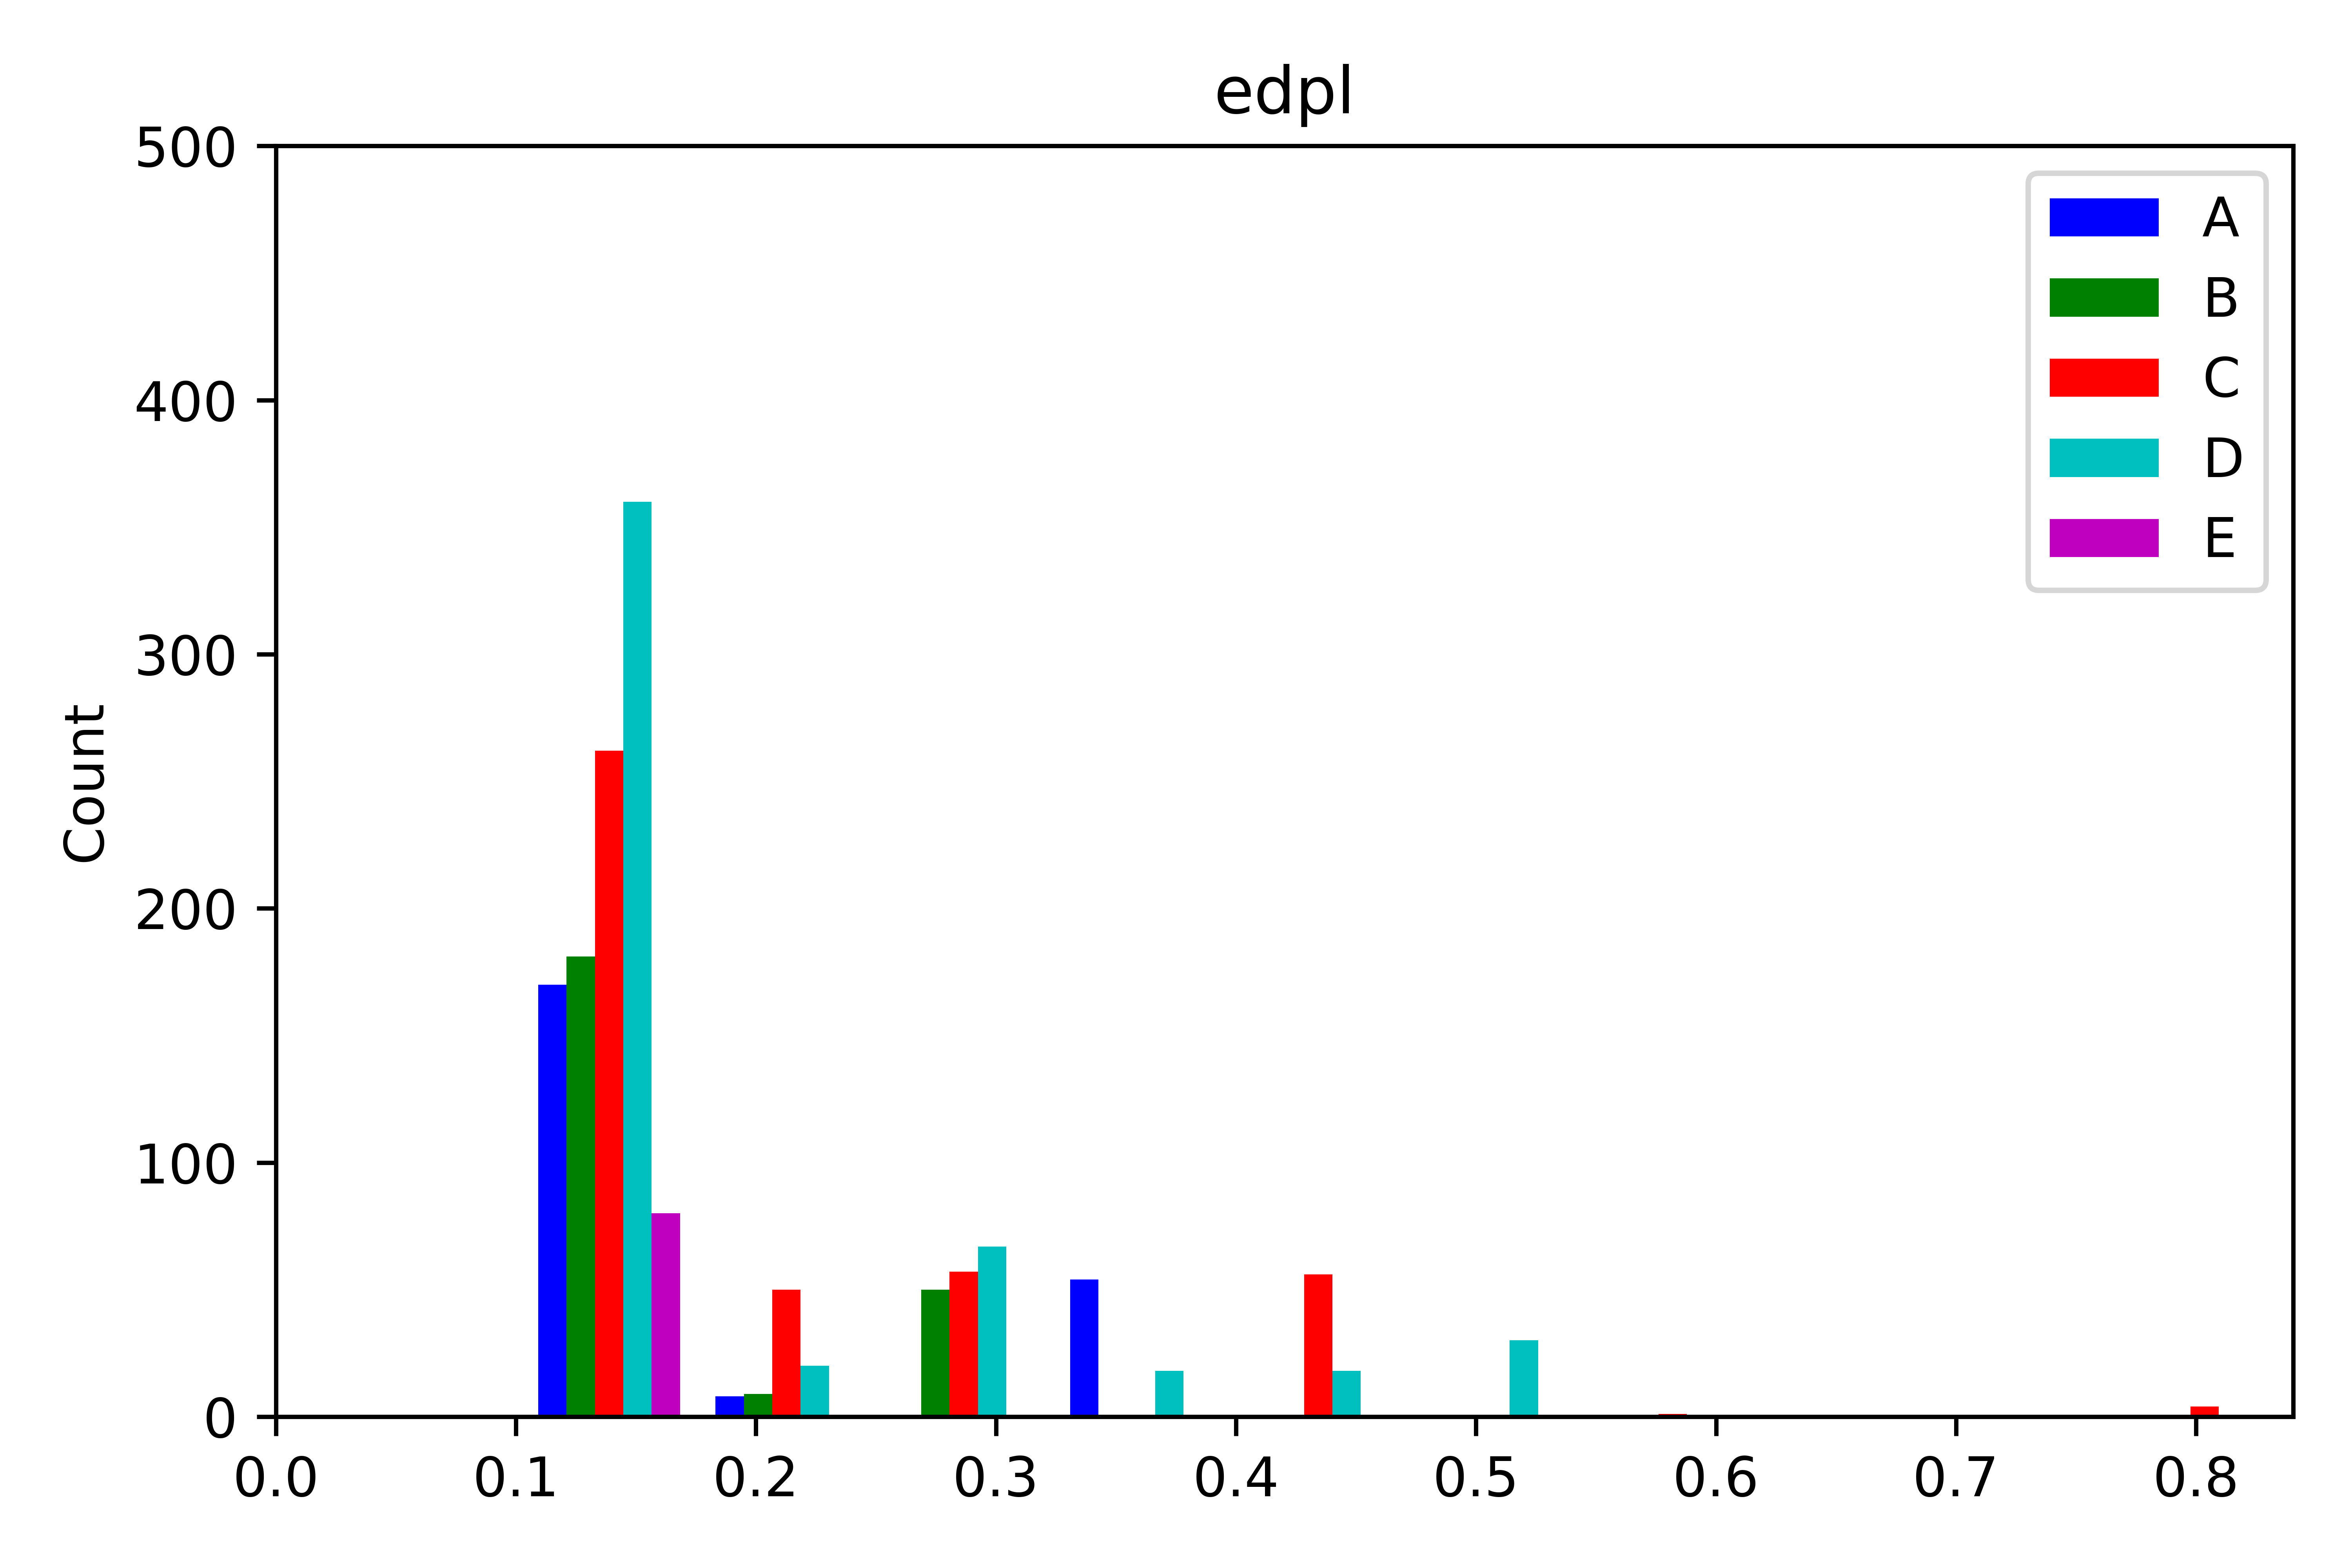
\includegraphics[width=\textwidth, keepaspectratio]{edpl.png}\\
	\caption{edpl distribution}
	\label{edpl}
\end{figure}


prichness, shown as in Figure \ref{prichness} \par
\begin{figure}[H]
	\centering
	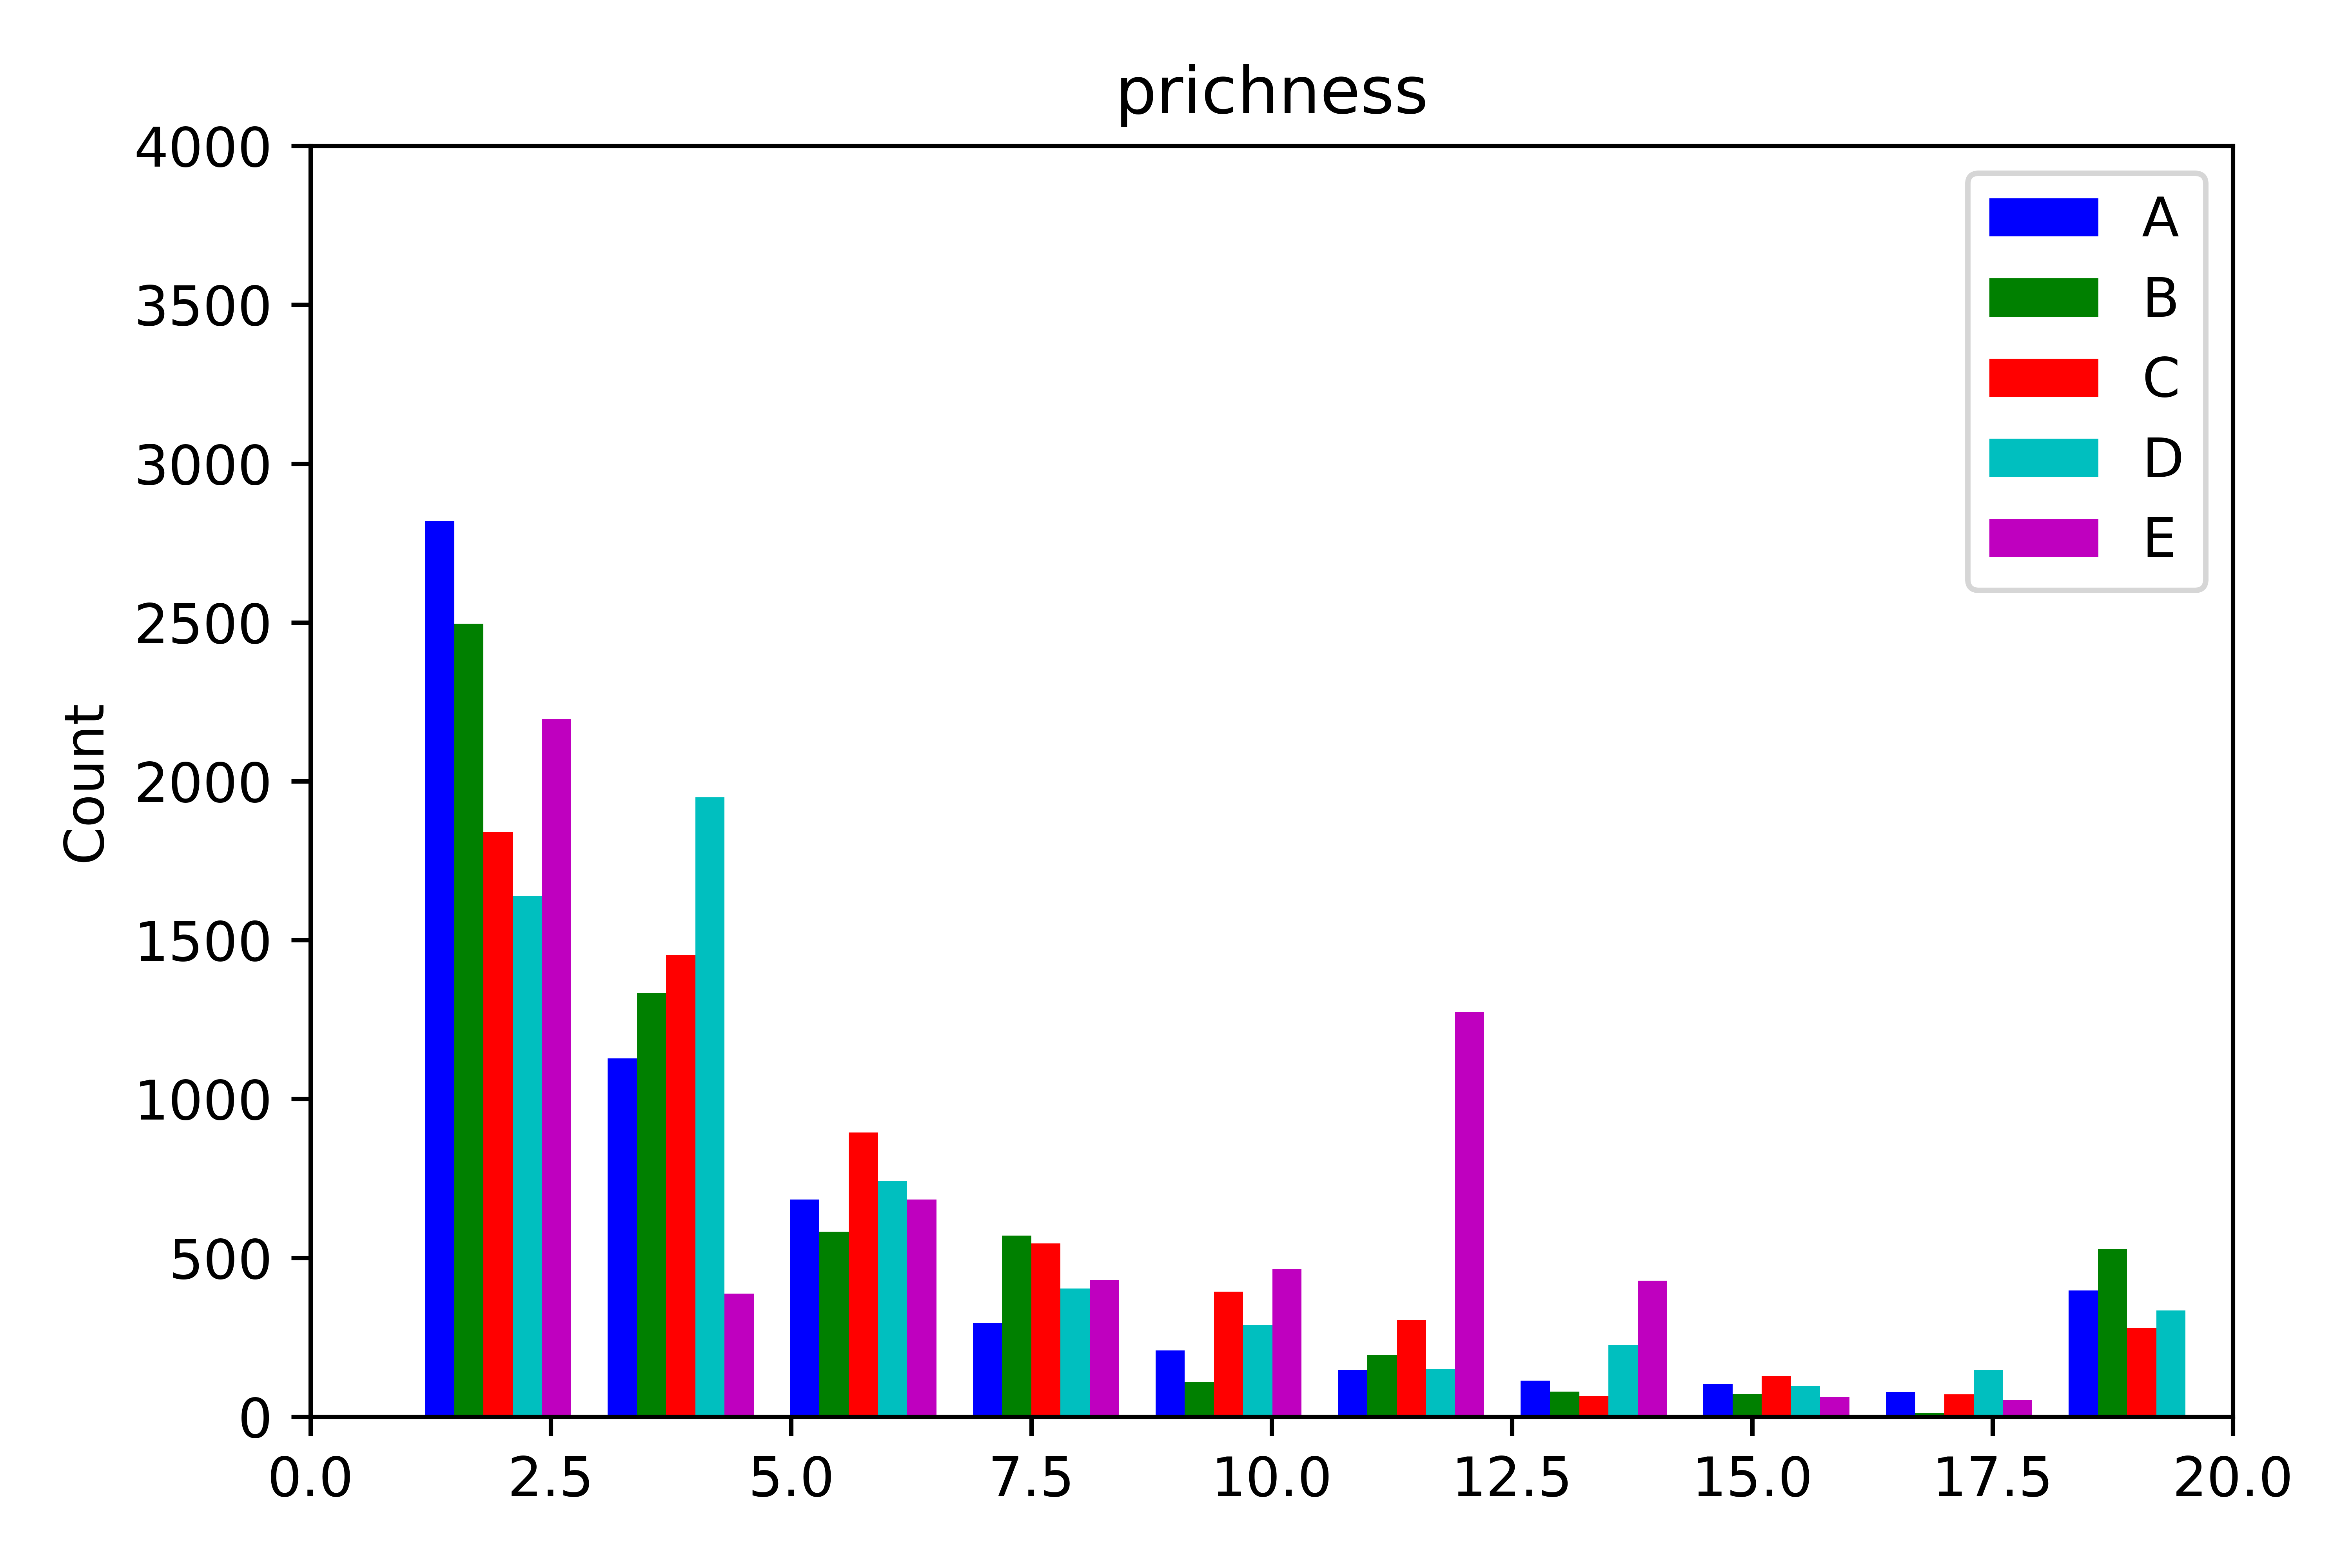
\includegraphics[width=\textwidth, keepaspectratio]{prichness.png}\\
	\caption{prichness distribution}
	\label{prichness}
\end{figure}


mindistl, shown as in Figure \ref{mindistl}
\begin{figure}[H]
	\centering
	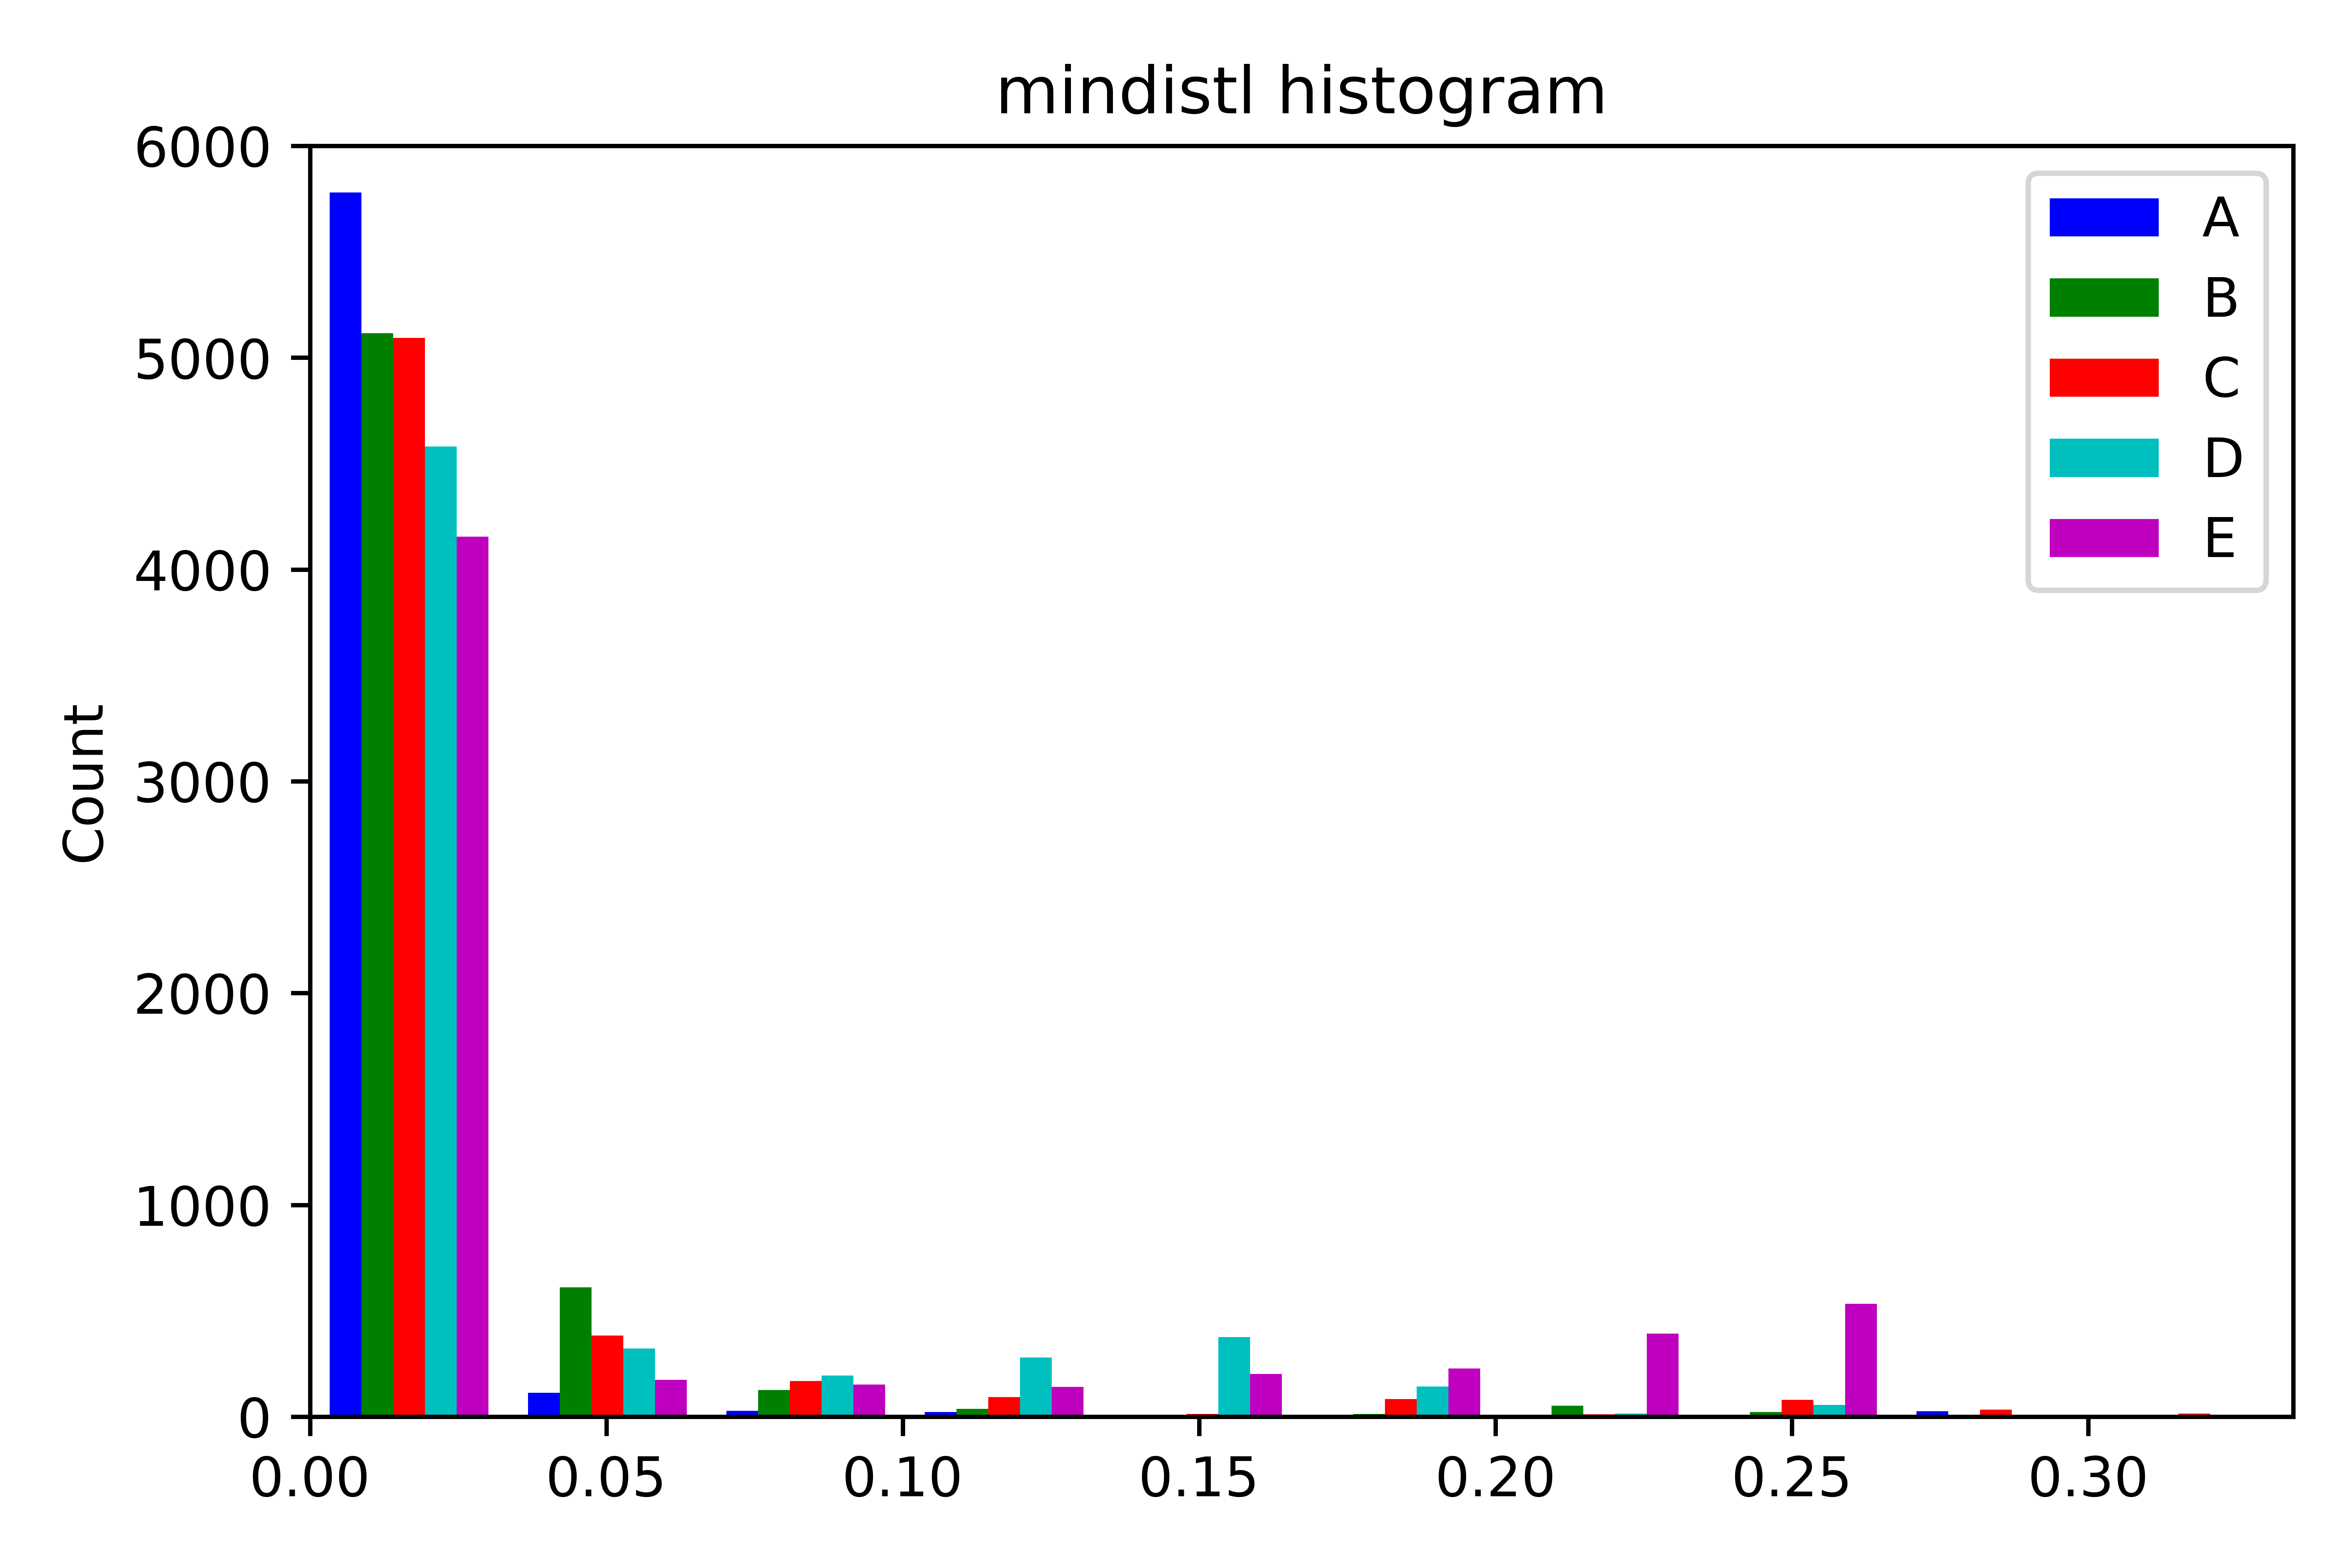
\includegraphics[width=\textwidth, keepaspectratio]{mindistl.png}\\
	\caption{mindistl distribution}
	\label{mindistl}
\end{figure}


\end{document}